% for hyperref color change to RoyalBlue4
\PassOptionsToPackage{svgnames,x11names}{xcolor}
\documentclass[11pt]{article}

% general styling
\usepackage{UF_FRED_paper_style}
% for header in title page
\usepackage{fancyhdr}
\pagestyle{fancy}
\lhead{}
\rhead{}
\chead{}
\renewcommand{\headrulewidth}{0pt}
\fancypagestyle{firstpage}{%
  \lhead{\large{RESEARCH REPORT}}
  \setlength{\headheight}{14pt} 
  \renewcommand{\headrulewidth}{1.2pt}
  \rhead{}
}

\usepackage{apacite}
\usepackage{txfonts} %for edge-endpoints
\usepackage{tikz}
% \usepackage[capposition=bottom]{floatrow}
\usepackage[format=plain,
            labelfont={it}, singlelinecheck=false,
            justification = raggedright,
            labelsep = period,
            figureposition=top]{caption}
\usepackage{algorithm}
\usepackage{algcompatible}
\usepackage{algpseudocode}
\usepackage{amssymb}
\usepackage{amsmath}
\usepackage{mathtools}
% for appendix title
\usepackage[title]{appendix}
 % to remove space between enumerate items
\usepackage{enumitem}
% to specify a different margin for a page
\usepackage{afterpage}
%for table
\usepackage{tabularx, multirow,booktabs,setspace,caption}
\usepackage{tabularray}
%\usepackage[hmargin=1cm]{geometry}
% for adding affiliation
\usepackage{authblk} 
% for the adjustwidth environment
\usepackage{changepage} 
% for space between text and footnote
\setlength{\skip\footins}{1.2pc plus 5pt minus 2pt}
% hyperlink
\usepackage{hyperref} 
\hypersetup{
    colorlinks=true,
    linkcolor= MidnightBlue,
    filecolor= MidnightBlue,      
    urlcolor= MidnightBlue,
    pdftitle={Research Report Kyuri Park},
    citecolor= MidnightBlue,
    pdfpagemode=FullScreen
    }


%% for (in)dependence symbols
\makeatletter
\newcommand\multiline[1]{\parbox[t]{\dimexpr\linewidth-\ALG@thistlm}{#1}}
\makeatother

%% (in)dependence symbol
\usepackage{unicode-math}

\makeatletter
\newcommand*{\indep}{%
  \mathbin{%
    \mathpalette{\@indep}{}%
  }%
}
\newcommand*{\nindep}{%
  \mathbin{%                  % The final symbol is a binary math operator
    %\mathpalette{\@indep}{\not}% \mathpalette helps for the adaptation
    \mathpalette{\@indep}{/}%
                               % of the symbol to the different math styles.
  }%
}
\newcommand*{\@indep}[2]{%
  % #1: math style
  % #2: empty or \not
  \sbox0{$#1\perp\m@th$}%        box 0 contains \perp symbol
  \sbox2{$#1=$}%                 box 2 for the height of =
  \sbox4{$#1\vcenter{}$}%        box 4 for the height of the math axis
  \rlap{\copy0}%                 first \perp
  \dimen@=\dimexpr\ht2-\ht4-.2pt\relax
      % The equals symbol is centered around the math axis.
      % The following equations are used to calculate the
      % right shift of the second \perp:
      % [1] ht(equals) - ht(math_axis) = line_width + 0.5 gap
      % [2] right_shift(second_perp) = line_width + gap
      % The line width is approximated by the default line width of 0.4pt
  \kern\dimen@
  \ifx\\#2\\%
  \else
    \hbox to \wd2{\hss$#1#2\m@th$\hss}%
    \kern-\wd2 %
  \fi
  \kern\dimen@
  \copy0 %                       second \perp
}
\makeatother
%%%%%%%%%%%%%

%% dotted underline
\newcommand{\udensdot}[1]{%
    \tikz[baseline=(todotted.base)]{
        \node[inner sep=1pt,outer sep=0pt] (todotted) {#1};
        \draw[densely dotted, thick] (todotted.south west) -- (todotted.south east);
    }%
}%


%% make cross sign for the table
\newcommand{\tikzxmark}{%
\tikz[scale=0.23] {
    \draw[line width=0.7,line cap=round] (0,0) to [bend left=6] (1,1);
    \draw[line width=0.7,line cap=round] (0.2,0.95) to [bend right=3] (0.8,0.05);
}}

%% for circle-arrow edge-endpoints
\def\leftcirc#1{% Parameter, arrow style
\xdef\y{0}
\foreach \left in {white} {
   {
    \draw[fill=\left]  (0,\y) circle (2pt);    
    \draw[shorten <=2pt, shorten >=2pt, arrows=#1] (0,\y) -- (0.7, \y);
    \pgfmathparse{\y+1}
    \global\let\y\pgfmathresult
  }
 }
}

\def\rightcirc#1{% Parameter, arrow style
\xdef\y{0}
 {
  \foreach \right in {white} {
    \draw[fill=\right] (0.7,\y) circle (2pt);
    \draw[shorten <=2pt, shorten >=2pt, arrows=#1] (0,\y) -- (0.7, \y);
    \pgfmathparse{\y+1}
    \global\let\y\pgfmathresult
  }
 }
}

% to extend hypoerref link to Figure and a, b, c
\newcommand*{\figref}[2][]{%
  \hyperref[{fig:#2}]{%
    Figure~\ref*{fig:#2}%
    \ifx\\#1\\%
    \else
      #1%
    \fi
  }%
}


% \usepackage[compatible]{algpseudocode}


% \theoremstyle{definition}
\newtheorem{definition}{Definition}

%use next two lines instead for non-italic alternative
%\newtheorem{preremark}{Definition}
%\newenvironment{mydef}{\begin{preremark}\upshape}{\end{preremark}}

% for reference list doi styling
\newcommand*{\doi}{}
\renewcommand{\doiprefix}{}
\makeatletter
\newcommand{\doi@}[1]{\urlstyle{same}\url{https://doi.org/#1}}
\DeclareRobustCommand{\doi}{\hyper@normalise\doi@}
\makeatother

%% ===============================================
%% Setting the line spacing (3 options: only pick one)
% \doublespacing
% \singlespacing
\onehalfspacing
%% ===============================================

\setlength{\droptitle}{-4em} %% Don't touch

% %%%%%%%%%%%%%%%%%%%%%%%%%%%%%%%%%%%%%%%%%%%%%%%%%%%%%%%%%%
% SET THE TITLE
% %%%%%%%%%%%%%%%%%%%%%%%%%%%%%%%%%%%%%%%%%%%%%%%%%%%%%%%%%%

% TITLE:
\title{Discovering Cyclic Causal Models in Psychological Research 
}


% AUTHOR:
\author[1]{\Large{Kyuri Park\thanks{Correspondence concerning this paper should be addressed to: Kyuri Park, Department of Methodology and Statistics, Utrecht University, Padualaan 14, 3584 CH Utrecht, The Netherlands. e-mail: \color{MidnightBlue}k.park@uu.nl}}\\
\large{Supervisor: Dr. Ois\'{i}n Ryan}}

\affil[1]{Department of Methodology and Statistics, Utrecht University}%



% DATE:
\date{\today}

% %%%%%%%%%%%%%%%%%%%%%%%%%%%%%%%%%%%%%%%%%%%%%%%%%%%%%%%%%%
% %%%%%%%%%%%%%%%%%%%%%%%%%%%%%%%%%%%%%%%%%%%%%%%%%%%%%%%%%%
\begin{document}

\maketitle
\thispagestyle{firstpage}

\begin{adjustwidth}{1.5cm}{1.5cm}
{\setstretch{0.8}
\noindent This research report is written as a \textit{half of the thesis} format, including the introduction, background, and methods section along with the references and appendices at the end. The candidate journal for publication is \textit{Psychological Methods}.\\
\noindent\textbf{\textit{Keywords: }}%
cyclic causal discovery, causal inference, directed cyclic graph\\
\noindent\textbf{\textit{Word count: }}%
2499}
\end{adjustwidth}


% %%%%%%%%%%%%%%%%%%%%%%%%%%%%%%%%%%%%%%%%%%%%%%%%%%%%%%%%%%
% %%%%%%%%%%%%%%%%%%%%%%%%%%%%%%%%%%%%%%%%%%%%%%%%%%%%%%%%%%
% BODY OF THE DOCUMENT
% %%%%%%%%%%%%%%%%%%%%%%%%%%%%%%%%%%%%%%%%%%%%%%%%%%%%%%%%%%
% %%%%%%%%%%%%%%%%%%%%%%%%%%%%%%%%%%%%%%%%%%%%%%%%%%%%%%%%%%

% --------------------
\section{Introduction}
% --------------------
A fundamental task in various disciplines of science is to understand the mechanisms, that is, causal relations underlying the phenomena of interest. In psychology, for example, one of the core questions is how psychopathology comes about, with the network theory positing that mental disorder is produced by a system of direct causal interactions between symptoms \citep{BorsboomCramer2013}. In practice, empirical researchers often aim to gain insights into these causal relations by fitting statistical network models to observational data, an approach that can be characterized as a form of causal discovery \citep{spirtes2000}. However, it has been shown that network models are likely to perform poorly as causal discovery tools; relations in the network may not reflect the direct causal effects that researchers aim to discover, but can instead be produced by unwittingly conditioning on common effects or by failing to account for unobserved confounders \citep{dablander2019node, Ryan2022}.

In the field of causal discovery, using statistical independencies estimated from observational data to infer causal structures is known as \textit{constraint-based} causal discovery \citep{spirtes_algorithm_1991}. \cite{Ryan2022} suggest that network models could be replaced by purpose-built constraint-based causal discovery methods. However, the most popular and well-studied constraint-based methods assume that causal relationships are \textit{acyclic}; if X causes Y, then Y does not cause X \citep{Glymour2019}. This is problematic since \textit{cyclic} relationships or \textit{feedback loops} are critical to the theoretical understanding of psychopathology \citep{borsboom_network_2017}. For example, \cite{wittenborn_2016} suggest that several different causal feedback loops, such as \textit{perceived stress $\rightarrow$ negative affect $\rightarrow$ rumination $\rightarrow$ perceived stress} play a key role in sustaining depression. Such theoretical expectations necessitate the use of \textit{cyclic causal discovery} methods. Although some cyclic causal discovery algorithms have been developed \citep{mooij_classen2020}, they have not been as well studied as their acyclic counterparts, which is in part due to practical difficulties in fitting and interpreting cyclic causal models. To our knowledge, little to no research has been done on the applicability of cyclic causal discovery methods in psychology, and much remains unknown about the performance of these methods.

% Such theoretical expectations necessitate the use of \textit{cyclic causal discovery} algorithms. Although a number of cyclic causal discovery algorithms have been developed \citep{mooij_classen2020}, they have not been as well studied as their acyclic counterparts. In part this is due to practical difficulties in fitting and interpreting cyclic causal models.
% While other cyclic causal discovery techniques have recently been applied in psychological settings \citep{Kossakowski2021}, these methods require a mix of experimental data from different settings, a disadvantage when compared to constraint-based methods. To our knowledge, little to no research has been done on the applicability of constraint-based cyclic causal discovery algorithms in psychological research. 
Therefore, in this paper, we aim to address the following question: how well do
cyclic causal discovery methods perform in typical psychological research contexts? The goal of this study is twofold. First, we provide an accessible overview of different cyclic causal discovery methods. Second, we investigate how well each of these methods works by means of a simulation study.  
% Hence, in this paper, we aim to examine the suitability of cyclic causal discovery methods for psychological research. The goal of this study is twofold. First, we provide an accessible overview of different cyclic causal discovery methods. Second, we investigate how well each of these methods works by means of a simulation study. 
% \vspace{-3mm}

% In this paper, we investigate the suitability of cyclic causal discovery methods for psychological research. The goal of this study is twofold; First, we will provide an accessible overview of different cyclic causal discovery methods, including the assumptions under which they are expected to work. Second, we will investigate how well each of these methods works by means of a simulation study, where we vary the sample size, network size, network density, and presence of unobserved confounding. 


% Such theoretical expectations necessitate the use of more complex \textit{cyclic causal discovery} algorithms. Although a number of cyclic causal discovery algorithms have been developed \citep{mooij_classen2020}, they have not been as well studied as their acyclic counterparts. In part this is due to practical difficulties in fitting and interpreting cyclic causal models, since the properties, which map statistical to causal (in)dependencies are more complex than for acyclic models. While other cyclic causal discovery techniques have recently been applied in psychological settings \citep{Kossakowski2021}, these methods require a mix of experimental data from different settings, a disadvantage when compared to constraint-based methods. To our knowledge, little to no research has been done on the applicability of constraint-based cyclic causal discovery algorithms in psychological research. 

% In this paper, we investigate the suitability of cyclic causal discovery methods for psychological research. The goal of this study is twofold; First, we will provide an accessible overview of different cyclic causal discovery methods, including the assumptions under which they are expected to work. Second, we will investigate how well each of these methods works by means of a simulation study, where we vary sample size, network size, density of the causal relations, and the presence of unobserved confounding. 

% Third, we will demonstrate their applicability in practice by testing them on empirical psychological data.

% We choose three algorithms that can handle cyclic structure: cyclic causal discovery (CCD), cyclic causal inference (CCI), fast causal inference (FCI).


\section{Background}
In this section, we introduce the basic concepts of graphical models, which are necessary to understand the causal discovery methods that we will study in the remainder of this paper. 
% \vspace{-3mm}
\subsection{Graphical Models} 
\vspace{-1mm}
% A graphical model is a set of multivariate joint distributions that show certain conditional independencies among random variables. Each model is associated with a graph $G = (V, E)$, where $V$ represents a set of vertices (nodes) and $E$ represents a set of edges that encode the conditional independencies between each pair of vertices (ref). 
% We use the term causal graphical model to denote a graphical model that describes the causal mechanisms of a system. 
% Causal graphical models can capture the probabilistic and causal properties of multivariate distributions, under the two following assumptions.

A graph ($\mathcal{G}$) is a diagram made up of a set of vertices ($\mathcal{V}$) and edges ($\mathcal{E}$), describing connections between vertices, denoted as $\mathcal{G} = (\mathcal{V},  \mathcal{E})$.
A probabilistic graphical model uses a graph to express the conditional (in)dependencies between random variables, where the vertices represent random variables, and the edges encode conditional dependencies holding among the set of variables \citep{lauritzen1996graphical}. 
% There exist various graphical models, typically differing in the types of edges (e.g., directed vs. undirected), and the corresponding interpretation of edges in terms of statistical relationships. One of the most commonly known graphical models in psychology is the \textit{Pairwise Markov Random Field} (PMRF), which forms the basis of statistical network models. In PMRF networks, the edges are strictly undirected, and the presence of an edge $A-B$ represents that $A$ and $B$ are statistically dependent conditioning on the set of all other variables \citep{borsboom_network_2021}. 
In a \textit{causal} graphical model, on the other hand, the edges describe \textit{causal} relationships between variables; the edges are typically directed, with $A \rightarrow B$ denoting that intervening on $A$ results in a change in the probability distribution of $B$ \citep{geiger_logic_1990}. Two example causal graphical models are shown in \figref{1}. \figref[a]{1} does not contain any cycles, whereas \figref[b]{1} does, hence called a \textit{directed acyclic graph} (DAG) and \textit{directed cyclic graph} (DCG), respectively. 

Causal graphical models also describe patterns of statistical independencies, which can be read off from the graph using Pearl's \textit{d-separation criterion} \citep{geiger_d-separation_1990}. For instance, in \figref[a]{1}, we see a \textit{chain} structure $X_1 \rightarrow X_2 \rightarrow X_3$, which implies that $X_1$ and $X_3$ are marginally dependent ($X_1 \nindep X_3$), but independent conditional on $X_2$ ($X_1 \indep X_3 \mid X_2$). More formally, we would say $X_1$ and $X_3$ are \textit{d-separated} by $X_2$. A \textit{fork} structure $X_3 \leftarrow X_2 \rightarrow X_4$ implies the same pattern of independencies; $X_3$ and $X_4$ are marginally dependent ($X_3 \nindep X_4$), but independent conditional on $X_2$ ($X_3 \indep X_4 \mid X_2$). That is, $X_3$ and $X_4$ are \textit{d-connected} given an empty set, but \textit{d-separated} by $X_2$. However, a \textit{collider} structure $X_2 \rightarrow X_4 \leftarrow X_5$ implies a contrasting pattern; here $X_2$ and $X_5$ are marginally independent ($X_2 \indep X_5$), but dependent conditional on $X_4$ ($X_2 \nindep X_5 \mid X_4$). This distinguishing characteristic of colliders is crucial when identifying the directions of causal relations, as will be shown later in section \ref{primer}.

\begin{figure}[H]
    \centering
        \caption{Example causal graphical models.}
        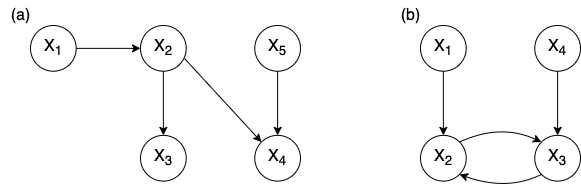
\includegraphics[scale=.5]{figures/DAG_DCG.png}
        \vspace{3mm}
        \caption*{\small{\textit{Note.} (a) is the example directed acyclic graph (DAG). (b) is the example directed cyclic graph (DCG).}}
    \label{fig:1}
\end{figure}


% One of the simplest and most well-known causal graphs is \textit{directed acyclic graph} (DAG), also known as \textit{Bayesian networks}, which consists of directed edges without cycles. In a DAG, a directed edge $A \rightarrow B$ indicates that $A$ is a direct cause of $B$.
\vspace{-0.8cm}
\subsection{Acyclic vs. Cyclic Causal Graphs} \label{acyclicvscyclic}

The d-separation criterion described above applies to all acyclic graphs, but only applies to graphs with cycles under certain conditions. To understand these conditions, first we need to introduce some graph terminology. We can use kinship terminology to describe a graph structure as follows:
\vspace{-0.1cm}
\begin{equation*}
\text{if }
  \begin{rcases}
    \begin{dcases}
      A \rightarrow B \\
      A \leftarrow B \\
      A \rightarrow \cdots \rightarrow B \,\,or \,\,A = B \\
      A \leftarrow \cdots \leftarrow B \,\,or \,\,A = B
\end{dcases}
  \end{rcases}
  \text{ in } \mathcal{G} \text{ then } A \text{ is a }
  \begin{rcases}
    \begin{dcases}
      \text{parent} \\
      \text{child} \\
      \text{ancestor} \\
      \text{descendant}
\end{dcases}
  \end{rcases}
\text{ of } B \text{ and}
  \begin{rcases}
    \begin{dcases}
      A \in pa_{\mathcal{G}}(B) \\
      A \in ch_{\mathcal{G}}(B) \\
      A \in an_{\mathcal{G}}(B) \\
      A \in de_{\mathcal{G}}(B)
\end{dcases}
  \end{rcases}
\text{.}
\end{equation*}

\noindent Also, when there exists an edge between two vertices $A - B$, $A$ and $B$ are said to be \textit{adjacent}. For example, in \figref[b]{1}, $X_1 \in pa_{\mathcal{G}} \,X_2$, $\,X_2 \in ch_{\mathcal{G}} \, X_1$, $\,\{X_1, X_2, X_3, X_4\} \in an_{\mathcal{G}}\,X_3$, $\,\{X_1, X_2, X_3\} \in de_{\mathcal{G}} \,X_1$, and $X_2$ is adjacent to $X_1$ and $X_3$. With this in place, we can define the \textit{global Markov} condition, which states that d-separation relations represented in causal graphs can be used to read off statistical independence relations such that:
% Second, we need to define the condition under which the d-separation criterion holds. This is known as the \textit{global Markov} condition, which states that the d-separation relations represented in causal graphs correspond to the statistical (in)dependencies such that: 
$$ \text{if } A \indep_{\mathcal{G}} B \mid C \Longrightarrow X_{A} \indep X_{B} \mid X_{C} \text{ for all subsets of } A, B, C, $$

\noindent where $\indep_{\mathcal{G}}$ refers to d-separation. If causal graphs are \textit{acyclic} (i.e., DAG), then the \textit{global Markov} condition holds regardless of the functional forms of causal relations and the distributions of variables involved \citep{lauritzen1996graphical}. In addition, in DAGs, the \textit{global Markov} condition also entails the \textit{local Markov} condition stating that a variable is independent of its non-descendants given its parents \citep{lauritzen2000graphical}. The fact that one Markov property instantly implies the other comes in handy when reading off conditional independencies from a graph.

In contrast to the acyclic case, the situation is not so straightforward in \textit{cyclic} graphs (i.e., DCG). In DCGs, the global Markov property does not always hold. \cite{spirtes1994}, in fact, showed that it holds for DCGs when causal relations are \textit{linear} and error terms are \textit{independent}. Furthermore, the local Markov property may not hold, even when the global Markov property holds. For example, in \figref[b]{1}, the global Markov property is preserved ($ X_1 \indep_{\mathcal{G}} X_4 \mid \{X_2, X_3\} \Longrightarrow X_{1} \indep X_{4} \mid \{X_2, X_3\}$), but the
local Markov property is violated as $X_2 \nindep_\mathcal{G} X_4 \mid X_3$ (i.e., $X_2$ is \textit{not} independent of its non-descendant $X_4$ given its parent $X_3$). This is because $X_3$ is both a parent of $X_2$ and a collider ($X_2 \rightarrow X_3 \leftarrow X_4$) at the same time.

Accordingly, we limit the scope of our study to cyclic causal graphs that represent \textit{linear} causal relationships with jointly \textit{independent} error terms, so for which the global Markov condition is satisfied. Additionally, we make use of one more assumption, known as \textit{faithfulness}, which is required for constraint-based causal discovery. 
\textit{Faithfulness} assumption is essentially the reverse of the global Markov condition, stating that statistical independencies map onto the structure of causal graphs such that:
$$ X_{A} \indep X_{B} \mid X_{C} \Longrightarrow A \indep_{\mathcal{G}} B \mid C.$$ Together with the global Markov property, faithfulness enables us to make inferences about causal relationships represented in graphs by testing for statistical independence among variables \citep{Bongers2021}.


% \subsection{Causal Modeling Assumptions}
% In order to map the relations represented in causal graphical models $\mathcal{G}$ to the structural functions in SCMs and vice versa, a couple of assumptions need to be satisfied; causal Markov assumption and faithfulness assumption.

% \subsubsection{Causal Markov Assumption} \label{markov}

% The causal Markov assumption is required when inferring a set of conditional independencies from a causal graphical model. It entails three Markov properties in specifics \citep{lauritzen1996graphical}. Given a directed graph $\mathcal{G}$ and a joint distribution $\mathcal{P}$, this distribution is said to satisfy:

% \begin{enumerate}[nolistsep]
%     \item \textit{global Markov} property if
%     $$ A \indep_{\mathcal{G}} B \mid C \Longrightarrow X_{A} \indep_{\mathcal{P}} X_{B} \mid X_{C}$$ for all subsets of $A$, $B$, $C$ (also known as the \textit{d-separation criterion}).

%     \item \textit{local Markov} property if each variable is independent of its non-descendants given its parents.

%     \item \textit{Markov factorization} property if  $$P(X_1, X_2, ..., X_n) = \prod_{i}^{n}P(\,X_i \,\,|\,\, pa_{i}^{\mathcal{G}}\,),$$ where $pa_{i}^{\mathcal{G}}$ denotes the \textit{parents} of node $i$ (factorization is equivalent to global Markov property when the distribution over $X$ has a density).
% \end{enumerate}


% \noindent The elegance of DAG is rooted in the equivalence of these various versions of Markov properties. When a DAG satisfies one of these Markov properties, it instantly implies that it satisfies the rest \citep{lauritzen2000graphical}. However, in directed cyclic graphs that is not the case. In fact, \cite{spirtes1994} showed that both global and local Markov properties may fail in directed graph with cycles.
% In the directed cyclic graph from Figure \ref{fig:1} (b) for example, it can be observed that global Markov property holds ($ X_1 \indep_{\mathcal{G}} X_4 \mid \{X_2, X_3\} \Longrightarrow X_{1} \indep_{\mathcal{P}} X_{4} \mid \{X_2, X_3\}$), but the
% local Markov property is violated as $X_1 \nindep_\mathcal{G} X_4 \mid X_2$ (i.e., $X_1$ is \textit{not} d-separated from its non-descendant $X_4$ given its parent $X_2$). On the contrary, it can be easily seen that all three properties hold in the DAG from Figure \ref{fig:1} (a).


% \subsubsection{Faithfulness Assumption}

% It states the reverse of causal Markov assumption. That is, a distribution $\mathcal{P}$ is faithful to a graph $\mathcal{G}$ if the conditional independencies imply the associated graph structure such that:

% $$ X_{A} \indep_{\mathcal{P}} X_{B} \mid X_{C} \Longrightarrow A \indep_{\mathcal{G}} B \mid C.$$
% Together with the global Markov property (i.e., d-separation criterion), faithfulness assumption is of key importance to infer causal relations from graphical models \citep{Bongers2021}.
 

% \subsubsection{Causal Models in Current Study} \label{currentscope}
% As the distribution $\mathcal{P}$ may not obey the global Markov property when $\mathcal{G}$ contains cycles, there has to be additional constraints imposed on $\mathcal{P}$ such that we can ensure that the property holds.
% Spirtes (1995) showed that if $\mathcal{P}$ obeys a linear SCM with jointly independent error terms ($\varepsilon$), then it satisfies the global Markov property with respect to the directed cyclic graph $\mathcal{G}$.
% Accordingly, here we limit the scope of our study to the subclass of cyclic SCMs, where the relationships between the variables are linear and the error terms are independent of each other. In addition, we assume that the error terms are normally distributed, which is one of common assumptions in psychological research \citep{zhang_statistical_2022}. 

\subsection{A Primer on Constraint-Based Causal Discovery} \label{primer}
Under the aforementioned assumptions, constraint-based methods seek to recover the underlying causal structure using conditional independencies estimated from observational data. Constraint-based methods typically employ a two-step procedure; (1) first, establishing the \textit{skeleton} -- an undirected version of the underlying graph -- and (2) second, attempting to assign directions to the edges. In general, constraint-based techniques are unable to uniquely identify the underlying causal graph, but instead return a set of causal graphs that imply the same statistical independence relations.

% By constraint-based, we mean a two-step procedure in which observed patterns of conditional independencies between variables are (1) first used to establish the \textit{skeleton} -- an undirected version of the underlying graph -- and (2) second, more detailed patterns are used to assign directions to edges. 

To develop an intuition for this, we examine how a constraint-based method works for the relatively simple DAG from \figref[a]{1}. We start with a fully-connected graph, as shown in \figref[a]{2}. In the first step, the \textit{skeleton} is estimated by testing for conditional independence; if two variables are independent when conditioning on any subset of the remaining variables (e.g., $ X_1 \indep X_3 \mid X_2,\, X_1 \indep X_4 \mid X_2, ...$), then the edge between the two variables is removed (see \figref[b]{2}). In the second step, (some) edges are oriented by searching for \textit{colliders} that induce distinctive patterns of independencies (e.g., $X_4$ is identified as a collider given $ X_2 \indep X_5 \text{ and } X_2 \nindep X_5 \mid X_4$, thus $X_2 \rightarrow X_4 \leftarrow X_5$ is oriented; see \figref[c]{2}).
% the algorithm searches for \textit{colliders} that induce distinctive patterns of (in)dependencies (e.g., $ X_2 \indep X_5 \text{ and } X_2 \nindep X_5 \mid X_4$) to orient edges (e.g., $X_2 \rightarrow X_4 \leftarrow X_5$; see \figref[c]{2}). 
Note that the resulting graph in \figref[c]{2} is not identical to the original true graph $\mathcal{G}$, as the two edges between $X_1 - X_2$ and $X_2 - X_3$ remain undirected. There are in fact three DAGs that are implied by the resulting graph, as shown in \figref{3}. These DAGs are called \textit{Markov equivalent}, meaning that they encode the same conditional independencies (i.e., the same d-separation relations hold), and we call such a set of equivalent graphs a \textit{Markov equivalence class}, denoted by $Equiv(\mathcal{G})$. This illustrates a general difficulty in constraint-based approach; there are usually multiple graphs that are consistent with an observed set of statistical independencies. Here, we described the constraint-based approach procedure for DAGs, but the same principles are adapted and used for cyclic graphs, which will be the focus of the remainder of this paper.\footnote{See \figref{3} for a summary of the constraint-based approach procedure.}

% Note that in this example we assumed another condition other than Markov and faithfulness assumptions, which was not explicitly stated above. We also relied on the assumption that there was no unobserved latent variables (i.e., \textit{causal sufficiency}). This illustrates the general difficulties of causal discovery methods; There are usually multiple causal graphs that are all consistent with the observed statistical independencies, and these methods often require more assumptions to work as they are intended. The causal discovery methods for \textit{cyclic} models also share these limitations and on top of that, relaxing acyclicity assumption adds more challenges. For instance, due to the fact that local Markov property does not hold in general in cyclic graphs, cyclic causal discovery methods often cannot infer the direct parental relationships, but only up to the ancestral relationships \citep{Bongers2021}. 

\pagebreak
\newgeometry{left=2.5cm,right=2.55cm,top=3cm,bottom=3cm}
% Also, we assumed that we had access to the correct conditional independence information, although in practice it might not be the case even when we perform an appropriate conditional independence test due to sampling error.

\begin{figure}[H]
    \centering
        \caption{Steps of a constraint-based method.}
        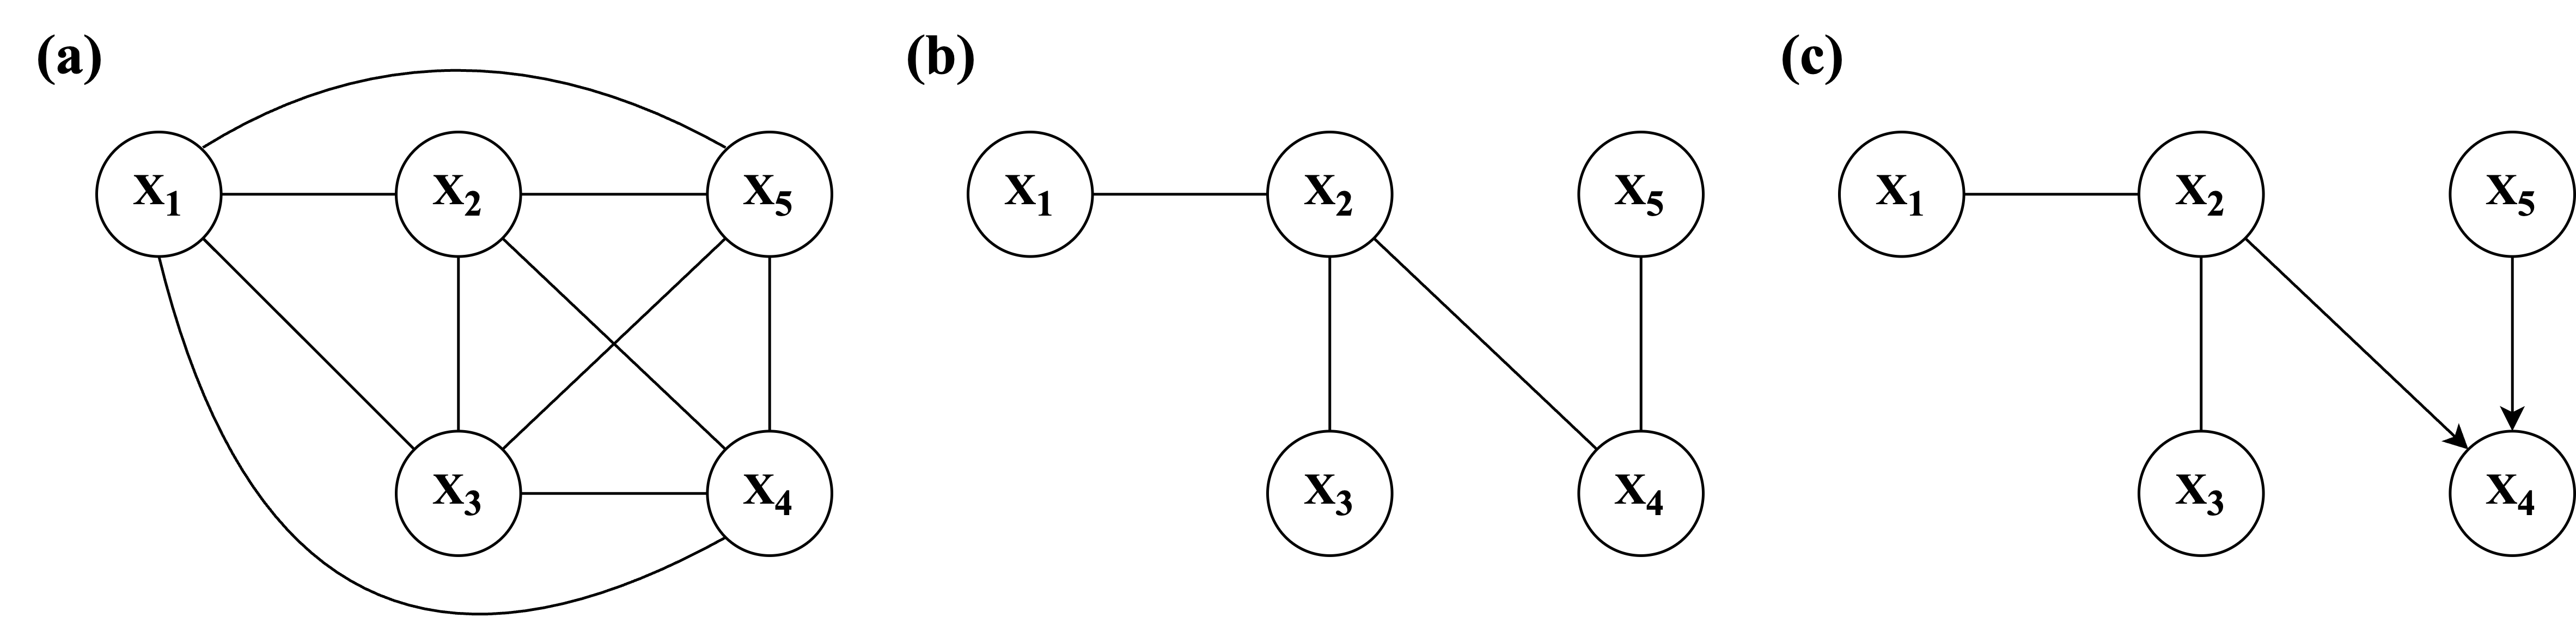
\includegraphics[width=1.0\textwidth]{figures/constraintstep.png}
        \vspace{0.1mm}
        \caption*{\small{\textit{Note.} (a) shows the fully-connected graph for the example DAG from \figref[a]{1}, which is the starting point. \\(b) shows the estimated \textit{skeleton} -- an undirected graph of the underlying causal structure -- after the first step. \\(c) shows the resulting graph after the second step, which represents the \textit{Markov equivalence class} of DAGs (i.e., a set of DAGs that entail the same set of conditional independencies).}}
    \label{fig:2}
\end{figure}


% \begin{figure}[H]
%     \centering
%         \caption{Markov equivalence set of DAGs}
%         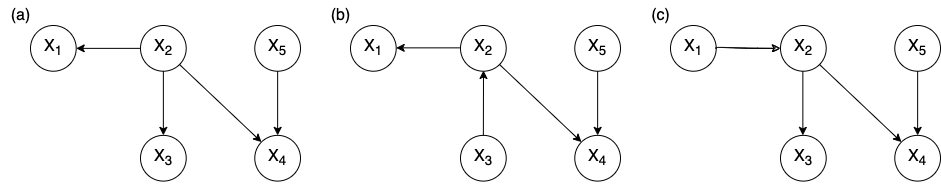
\includegraphics[width=1.0\textwidth]{figures/dag_equiv.png}
%     \label{fig:3}
% \end{figure}

\vspace{1cm}

\begin{figure}[H]
    \centering
        \caption{Summary of the constraint-based causal discovery procedure.}
        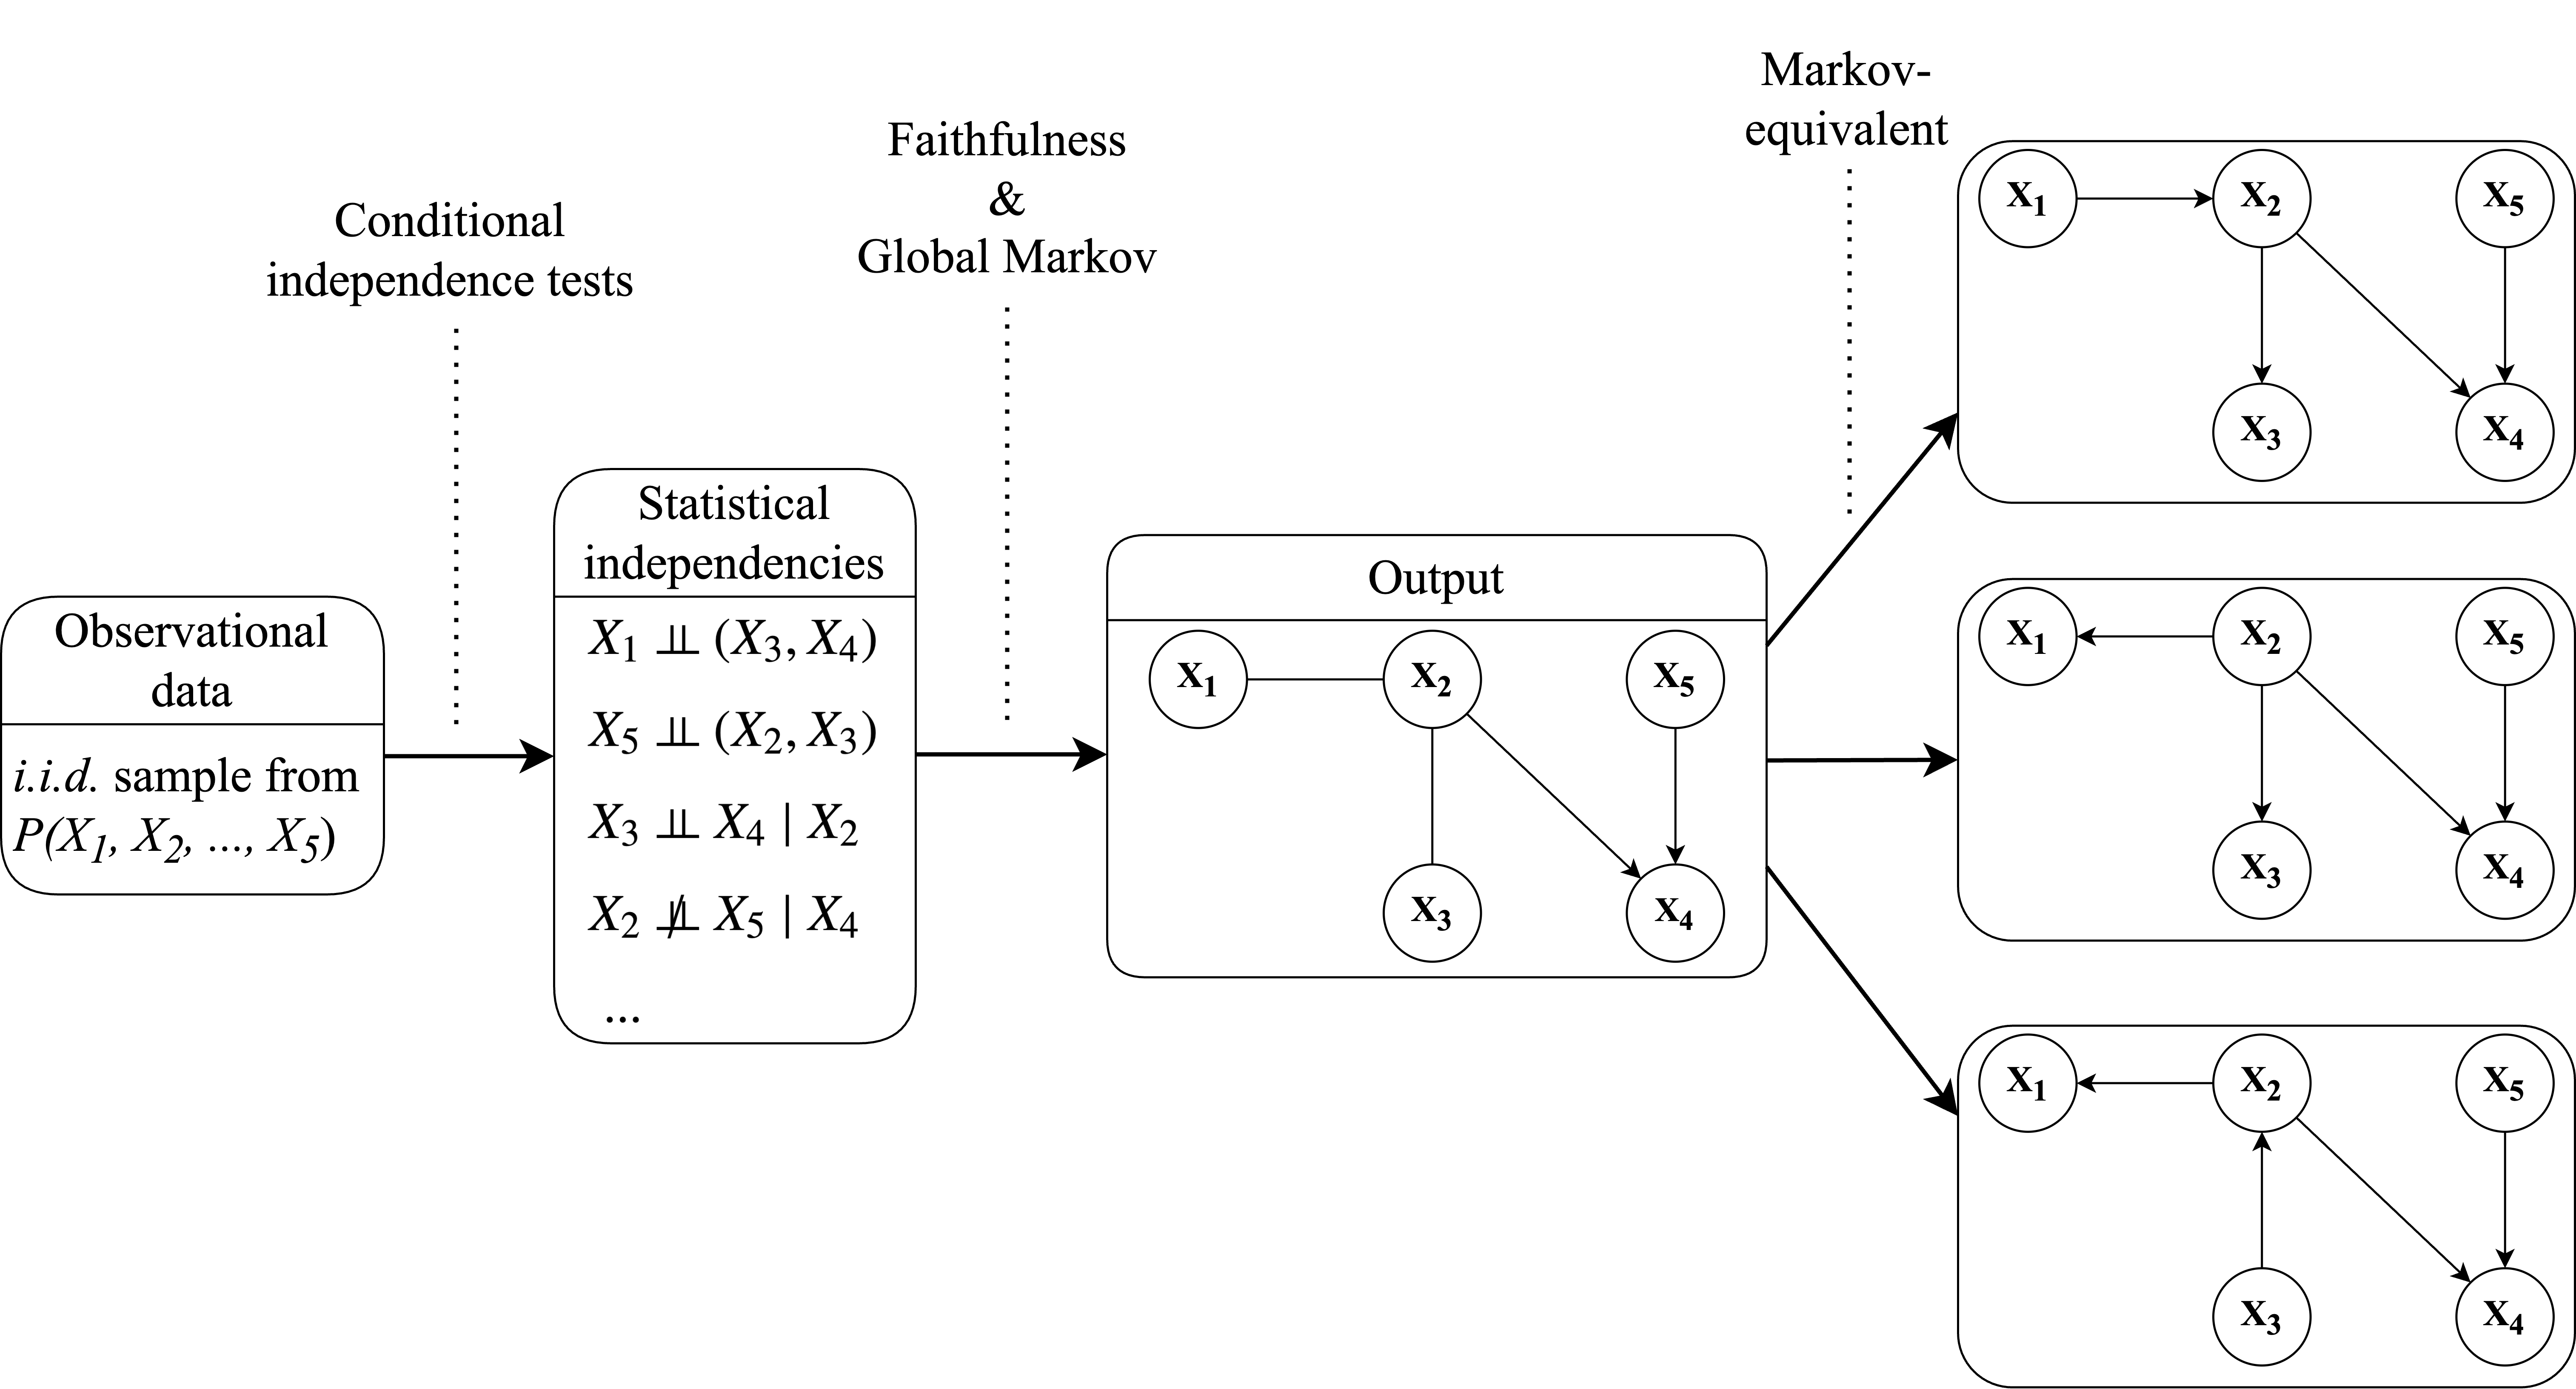
\includegraphics[width=1.0\textwidth]{figures/CB_summaryedited2.png}
        \vspace{0.1mm}
        \caption*{\small{\textit{Note.} A constraint-based algorithm starts with performing a series of conditional independence tests on observational (\textit{i.i.d.}: independent and identically distributed) data . Under the faithfulness and global Markov assumption, the algorithm estimates a graph structure based on the observed statistical independence patterns. \\The output is a \textit{partially directed} graph (as some edges remain undirected). It can represent multiple graphs that are \textit{Markov equivalent}, meaning that they imply the same statistical independence relations. This equivalent set of graphs is called \textit{Markov equivalence class}, and in this example, it consists of three different DAGs including the true DAG ($G$).}}
    \label{fig:3}
\end{figure}

% restore original geometry
\clearpage
\restoregeometry

\newpage
\section{Methods}
In this paper, we compare the performance of three different constraint-based algorithms for cyclic graphs using a simulation study: \textit{cyclic causal discovery} (CCD) \citep{Richardson1996a}, \textit{fast causal inference} (FCI) \citep{mooij_classen2020}, and \textit{cyclic causal inference} (CCI) \citep{strobl2019}. In this section, we provide a detailed description of one of the considered algorithms, CCD, and illustrate how we conduct the simulation study. The other two algorithms, FCI and CCI, work in a similar way, except that they do not require the assumption of \textit{no unobserved confounding} needed by the CCD algorithm.\footnote{The assumption that we have measured all common causes of variables involved.} (See \hyperref[algCCD]{Appendices} for the specifics of each of these three algorithms).

% except they do not assume that there are no unobserved latent confounders. See Appendices for the specifics of each of the three algorithms.

% In this paper, we compare the performance of three different constraint-based algorithms for cyclic models using a simulation study: \textit{cyclic causal discovery} (CCD) \citep{Richardson1996a}, \textit{fast causal inference} (FCI) \citep{mooij_classen2020}, and \textit{cyclic causal inference} (CCI) \citep{strobl2019}. In what follows, we first introduce the considered algorithms by describing the corresponding output and step-by-step tracing the algorithm. Then, we illustrate how we perform the simulation study, including the data generation process and evaluation metrics by which the performance is assessed. Given that all three algorithms work almost the same way, below we only provide a detailed description of the CCD algorithm\footnote{See Appendices for the specifics of each of the three algorithms.}.


% Table \ref{tab:1} summarizes the set of assumptions made by each of the algorithms. 

% \renewcommand{\tabularxcolumn}[1]{>{\centering\arraybackslash}p{#1}}
% \renewcommand{\arraystretch}{1.3}

% \begin{table}[ht]
% \caption{Overview of algorithms.}
% \label{tab:1}
% \begin{tabularx}{\textwidth}{p{5cm}*{3}{X}}
% \toprule
%  & CCD  & FCI & CCI \\

% \midrule
% Global Markov & \checkmark & \checkmark & \checkmark \\
% Faithfulness & \checkmark & \checkmark & \checkmark \\
% Acyclicity & \tikzxmark & \textendash $^a$ & \tikzxmark\\
% Causal sufficiency & \checkmark &  \tikzxmark &  \tikzxmark \\
% Linearity &  \checkmark & \tikzxmark &  \checkmark \\
% Independent errors & \checkmark & \checkmark & \checkmark\\
% \bottomrule

% \end{tabularx}

% \bigskip
% \small\textit{Note}. $^a$ FCI is originally designed assuming acyclicity, but in a recent research it has been proposed that it performs comparably well in the cyclic settings \citep{mooij_classen2020}.
% \end{table}


\subsection{CCD Algorithm}
In what follows, we introduce the type of output generated by the CCD algorithm and trace the algorithm step-by-step using an example. 

% In what follows, we explain how the CCD algorithm works by introducing the type of output generated by the algorithm and step-by-step tracing the algorithm using an example.
% CCD is a relatively simple causal discovery algorithm for cyclic models, as it assumes that there is no unobserved latent variables (i.e., \textit{causal sufficiency}). CCD algorithm can estimate the cyclic causal structure up to the equivalence class of graphs with the asymptotic correctness \citep{Richardson1996a}.

\subsubsection{Output Representation: Partial Ancestral Graph (PAG)}
% Previously in section \ref{primer}, we showed how a constraint-based method estimated a Markov equivalence class of DAGs. Here, we are interested in directed \textit{cyclic} graphs (DCG). 
As was the case with DAGs shown in section \ref{primer}, there typically exist multiple directed cyclic graphs (DCG) that imply the same statistical independencies, and so are statistically indistinguishable from one another. To represent a set of equivalent DCGs, a \textit{partial ancestral graph} (PAG) is used. Due to the possibility of cyclic relations, the causal semantics of edges in PAGs are more complicated; directed edges denote causal \textit{ancestry} (i.e., $A \rightarrow B$ means $A$ is an \textit{ancestor} of $B$), and there are three different types of edge-endpoints available: $\{ \circ, > , -  \}$. Additionally, a solid underlining or dotted underlining can be added in a PAG. In the following definition that provides the semantics for PAGs \citep{Richardson1996a}, $*$ is used as a \textit{meta-symbol} indicating one of the three possible edge-endpoints.\footnote{$A -*B$ indicates any of the following edges: $A-B$, $A\,->B$, or $A-\circ B$.}

% Previously in section \ref{primer}, we showed how a constraint-based method estimates a Markov equivalence class of DAGs. Here, we aim to find directed \textit{cyclic} graphs (DCG) and for that, we employ a \textit{partial ancestral graph} (PAG) to represent the Markov equivalence class of DCGs \citep{richardson1996}. Like a CPDAG, a PAG provides only \textit{partial} information on directions of the relations (i.e., some edges remain undirected) as there are many equivalent graphs exist based on the found statistical patterns. 
% To represent the equivalent set of cyclic graphs, we need a richer formalism than typical directed graphs. Accordingly, a PAG consists of a set of vertices, edges, and \textit{edge-endpoints} that are drawn from $\{ \circ, -, >, < \}$. $*$ is a so-called \textit{meta-symbol} that indicates one of the four possible edge-endpoints. In addition, a pair of edge-endpoints can be connected by either \textit{solid underlining} or \textit{dotted underlining}. 

\begin{definition} [PAG] \label{def: def2}
\textup{$\Psi$ is a PAG for a directed cyclic graph $\mathcal{G}$ iff:}
\begin{enumerate}[nolistsep]
    \item \textup{There is an edge between $A$ and $B$ in $\Psi$ iff $A$ and $B$ are d-connected in $\mathcal{G}$ given any subset of the remaining vertices.}
    
    \item \textup{If there is an edge $A -* B$ in $\Psi$, then $A$ is an ancestor of $B$ in every graph in an equivalence class, $Equiv(\mathcal{G})$.}

    \item \textup{If there is an edge $A *-> B$ in $\Psi$, then $B$ is \textit{not} an ancestor of $A$ in every graph in $Equiv(\mathcal{G})$.}

    \item \textup{If there is a solid underlining $A *-*\underline{B}*-*C$ in $\Psi$, then $B$ is an ancestor of (at least one of) $A$ or $C$ in every graph in $Equiv(\mathcal{G})$.}

    \item \textup{If there is a collider $A \rightarrow B \leftarrow C$, a dotted underlining is added $A \rightarrow \udensdot{B} \leftarrow C$ iff $B$ is \textit{not} a descendant of a common child of $A$ and $C$ in every graph in $Equiv(\mathcal{G})$.}
    % \udensdot{\textgreater B \textless}
    \item \textup{Any edge-endpoint not marked in one of the above ways is left with a circle $\circ-*$.}
    
\end{enumerate}
\end{definition}

\subsubsection{Steps of CCD Algorithm}
The CCD algorithm consists of 6 steps. We illustrate each step using the example DCG from \figref[a]{4}.\footnote{It is the same as the example DCG that we previously introduced in \figref[b]{1}.} The algorithm starts with a fully-connected PAG with circle endpoints, as shown in \figref[b]{4}, and as it proceeds (some) circles will be replaced by either an arrow head or a tail.\footnote{It is important to note, once again, that the algorithm aims to retrieve a PAG for the underlying cyclic graph, and the edges in a PAG represent \textit{ancestral} relations that are common to all directed cyclic graphs (DCG) in an equivalence class.}

\textbf{Step 1.} Estimate the \textit{ancestral} skeleton -- an undirected version of a PAG -- based on conditional independencies. When two vertices $A$ and $B$ are \textit{d-separated} given a set $S$, remove $A *-* B$ and record $S = \mathbf{Sepset} \langle A, B \rangle = \mathbf{Sepset} \langle B, A \rangle$. Since $X_1 \indep X_4 \mid \varnothing$ in our example DCG, $X_1 \multimapboth X_4$ is removed and $\mathbf{Sepset} \langle X_1, X_4 \rangle = \mathbf{Sepset} \langle X_4, X_1 \rangle = \varnothing$ is recorded, resulting in \figref[c]{4}.

\textbf{Step 2.} Search for collider structures. If $B \notin \mathbf{Sepset}\langle A, C \rangle$ in a triplet $A *-*B*-*C$, identify $B$ as a collider and orient $A \rightarrow B \leftarrow C$. Given that $X_2 \notin \mathbf{Sepset} \langle X_1, X_4 \rangle$ and $X_3 \notin \mathbf{Sepset} \langle X_1, X_4 \rangle$ in our example, $X_1 \multimapboth X_2 \multimapboth X_4$ and $X_1 \multimapboth X_3 \multimapboth X_4$ are oriented respectively as $X_1 \rightarrow X_2 \leftarrow X_4$ and $X_1 \rightarrow X_3 \leftarrow X_4$, resulting in \figref[d]{4}.

\textbf{Step 3.} Check for additional d-separating relations in each triplet $\langle A, B, C \rangle$ such that:\\
\textit{(i)} $A$ is not adjacent to $B$ or $C$,
\textit{(ii)} $B$ and $C$ are adjacent, and
 \textit{(iii)} $B \notin \mathbf{Sepset}\langle A, C \rangle$.
If such triplets exist, orient $B *-* C$ as $B \leftarrow C$. As no additional d-separating relations are found in our example, no further orientations are performed in step 3.
% such triplets are found in our example, no further orientations are performed in step 3.

\textbf{Step 4.} Search for $\mathbf{Supsets}$, which are d-separating sets including colliders. For each collider structure $A \rightarrow B \leftarrow C$, check if there is any set $T$ including $B$ that d-separates $A$ and $C$. When such exists, record $T = \mathbf{Supset} \langle A, B, C \rangle$ and add a dotted-underlining $A \rightarrow \udensdot{B} \leftarrow C$. Since $X_1 \indep X_4 \mid \{X_2, X_3\}$ in our example, $\mathbf{Supset}\langle X_1, X_2, X_4 \rangle = \mathbf{Supset}\langle X_1, X_3, X_4 \rangle = \{X_2, X_3\}$ is recorded and each of the colliders is dotted-underlined as $X_1 \rightarrow \udensdot{$X_2$} \leftarrow X_4$ and $X_1 \rightarrow \udensdot{$X_3$} \leftarrow X_4$, resulting in \figref[e]{4}.

\textbf{Step 5.} Search for quadruplets -- four ordered vertices $\langle A, B, C, D \rangle$ -- where:\\
\textit{(i)} $A \rightarrow \udensdot{B} \leftarrow C$, \textit{(ii)} $A \rightarrow D \leftarrow C$ or $A \rightarrow \udensdot{D} \leftarrow C$, and
\textit{(iii)} $B$ and $D$ are adjacent. 
If $D \in \mathbf{Supset} \langle A, B, C \rangle$ in such quadruplets, orient $B *-* D$ as $B *- D$. Else, orient $B *-* D$ as $B \rightarrow D$. In our example, there is such a quadruplet; \textit{(i)} $X_1 \rightarrow \udensdot{$X_2$} \leftarrow X_4$, \textit{(ii)} $X_1 \rightarrow \udensdot{$X_3$} \leftarrow X_4$, and \textit{(iii)} $X_2$ and $X_3$ are adjacent. Since $X_2 \in \mathbf{Supset} \langle X_1, X_3, X_4 \rangle$ and $X_3 \in \mathbf{Supset} \langle X_1, X_2, X_4 \rangle$, $X_2 \multimapboth X_3$ is oriented as $X_2 \multimap X_3$, then $X_2 \multimap X_3$ is subsequently oriented as  $X_2 - X_3$, resulting in \figref[f]{4}.

\textbf{Step 6.} Search for quadruplets $\langle A, B, C, D \rangle$, where $A \rightarrow \udensdot{B} \leftarrow C$ while $D$ is adjacent to neither $A$ nor $C$. If $A$ and $D$ are d-connected given $\mathbf{Supset} \langle A, B, C \rangle \cup {D}$, then orient $B * \multimap D$ as $B \rightarrow D$. In our example, no such quadruplets exist; therefore \figref[f]{4} remains the final PAG. As shown in \figref{5}, the resulting PAG represents two different DCGs that entail the same conditional independencies. 

\pagebreak
\newgeometry{left=2.5cm,right=2.7cm,top=2.5cm,bottom=3cm}

\begin{figure}[H]
    \centering
        \caption{Trace of CCD algorithm.}
        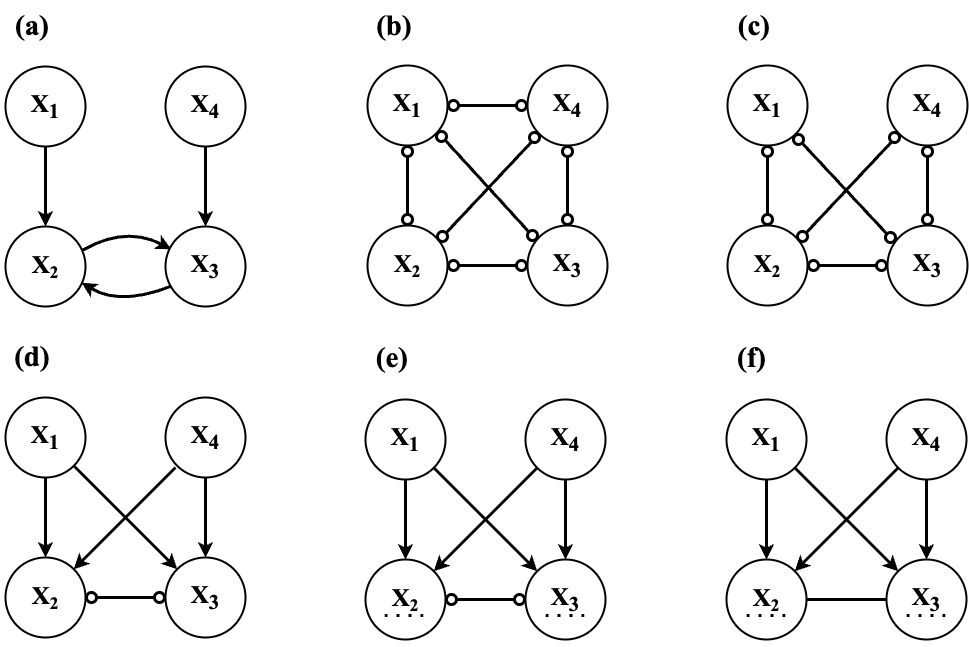
\includegraphics[width=.75\textwidth]{figures/ccdtrace_edited.png}
        \vspace{3mm}
        \caption*{\small{\textit{Note.} (a) shows the true directed cyclic graph, $\boldsymbol{G}$. (b) shows the fully-connected PAG for $\boldsymbol{G}$, which is the starting point of the algorithm. (c) shows the \textit{ancestral} skeleton (i.e., an undirected version of the PAG) estimated in step 1. (d) shows the state of the PAG after step 2, where some of the edges are oriented given the identified colliders. (e) shows the state of the PAG after step 4, where the \textit{Supsets} are identified and the corresponding colliders are dotted-underlined. (f) shows the final state of the PAG after step 5, where an additional edge between $X_2$ and $X_3$ is oriented.}}
    \label{fig:4}
\end{figure}

% Again, note that while the edges in $\boldsymbol{G}$ represent parental (i.e., direct causal) relations, the edges in PAGs represent \textit{ancestral} relations.

\begin{figure}[H]
    \centering
        \caption{Summary of CCD algorithm operation.}
        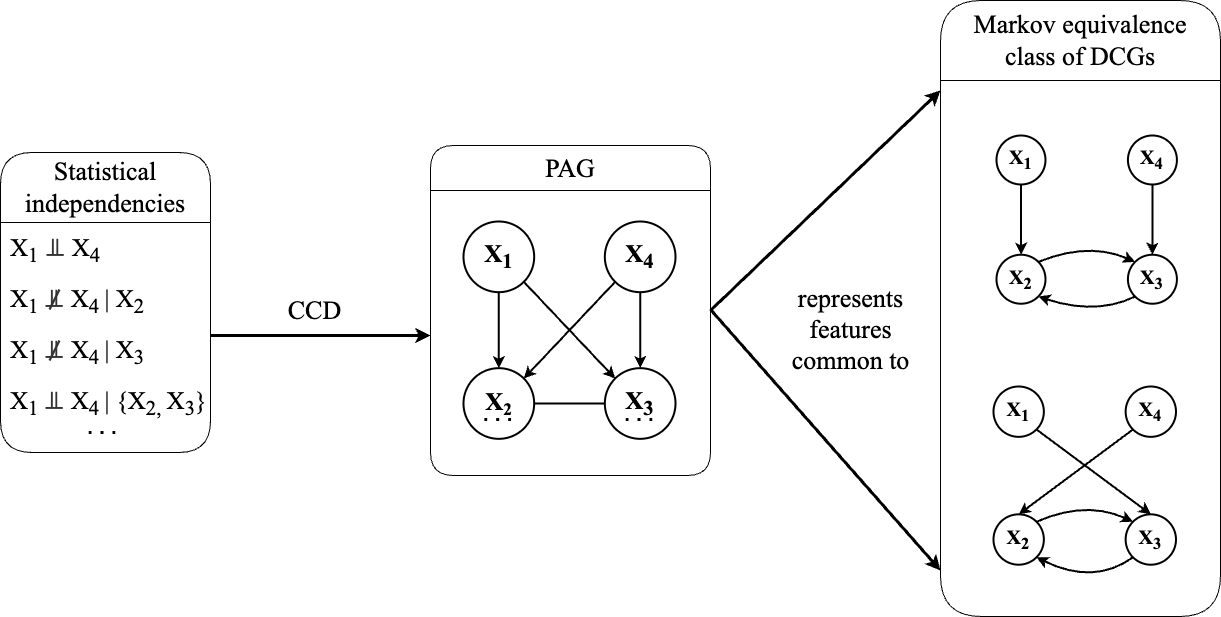
\includegraphics[width=1\textwidth]{figures/CCDsummaryedited.png}
        \vspace{3mm}
        \caption*{\small{\textit{Note.} Given the observed statistical independencies, CCD constructs a partial ancestral graph (PAG), which represents the \textit{ancestral} features that are common to every directed cyclic graph (DCG) in a Markov equivalence class. In this example, the Markov equivalence class consists of two different DCGs, including the true graph $\boldsymbol{G}$.}}
    \label{fig:5}
\end{figure}


% \begin{figure}[H]
%     \centering
%         \caption{Causal landscape.}
%         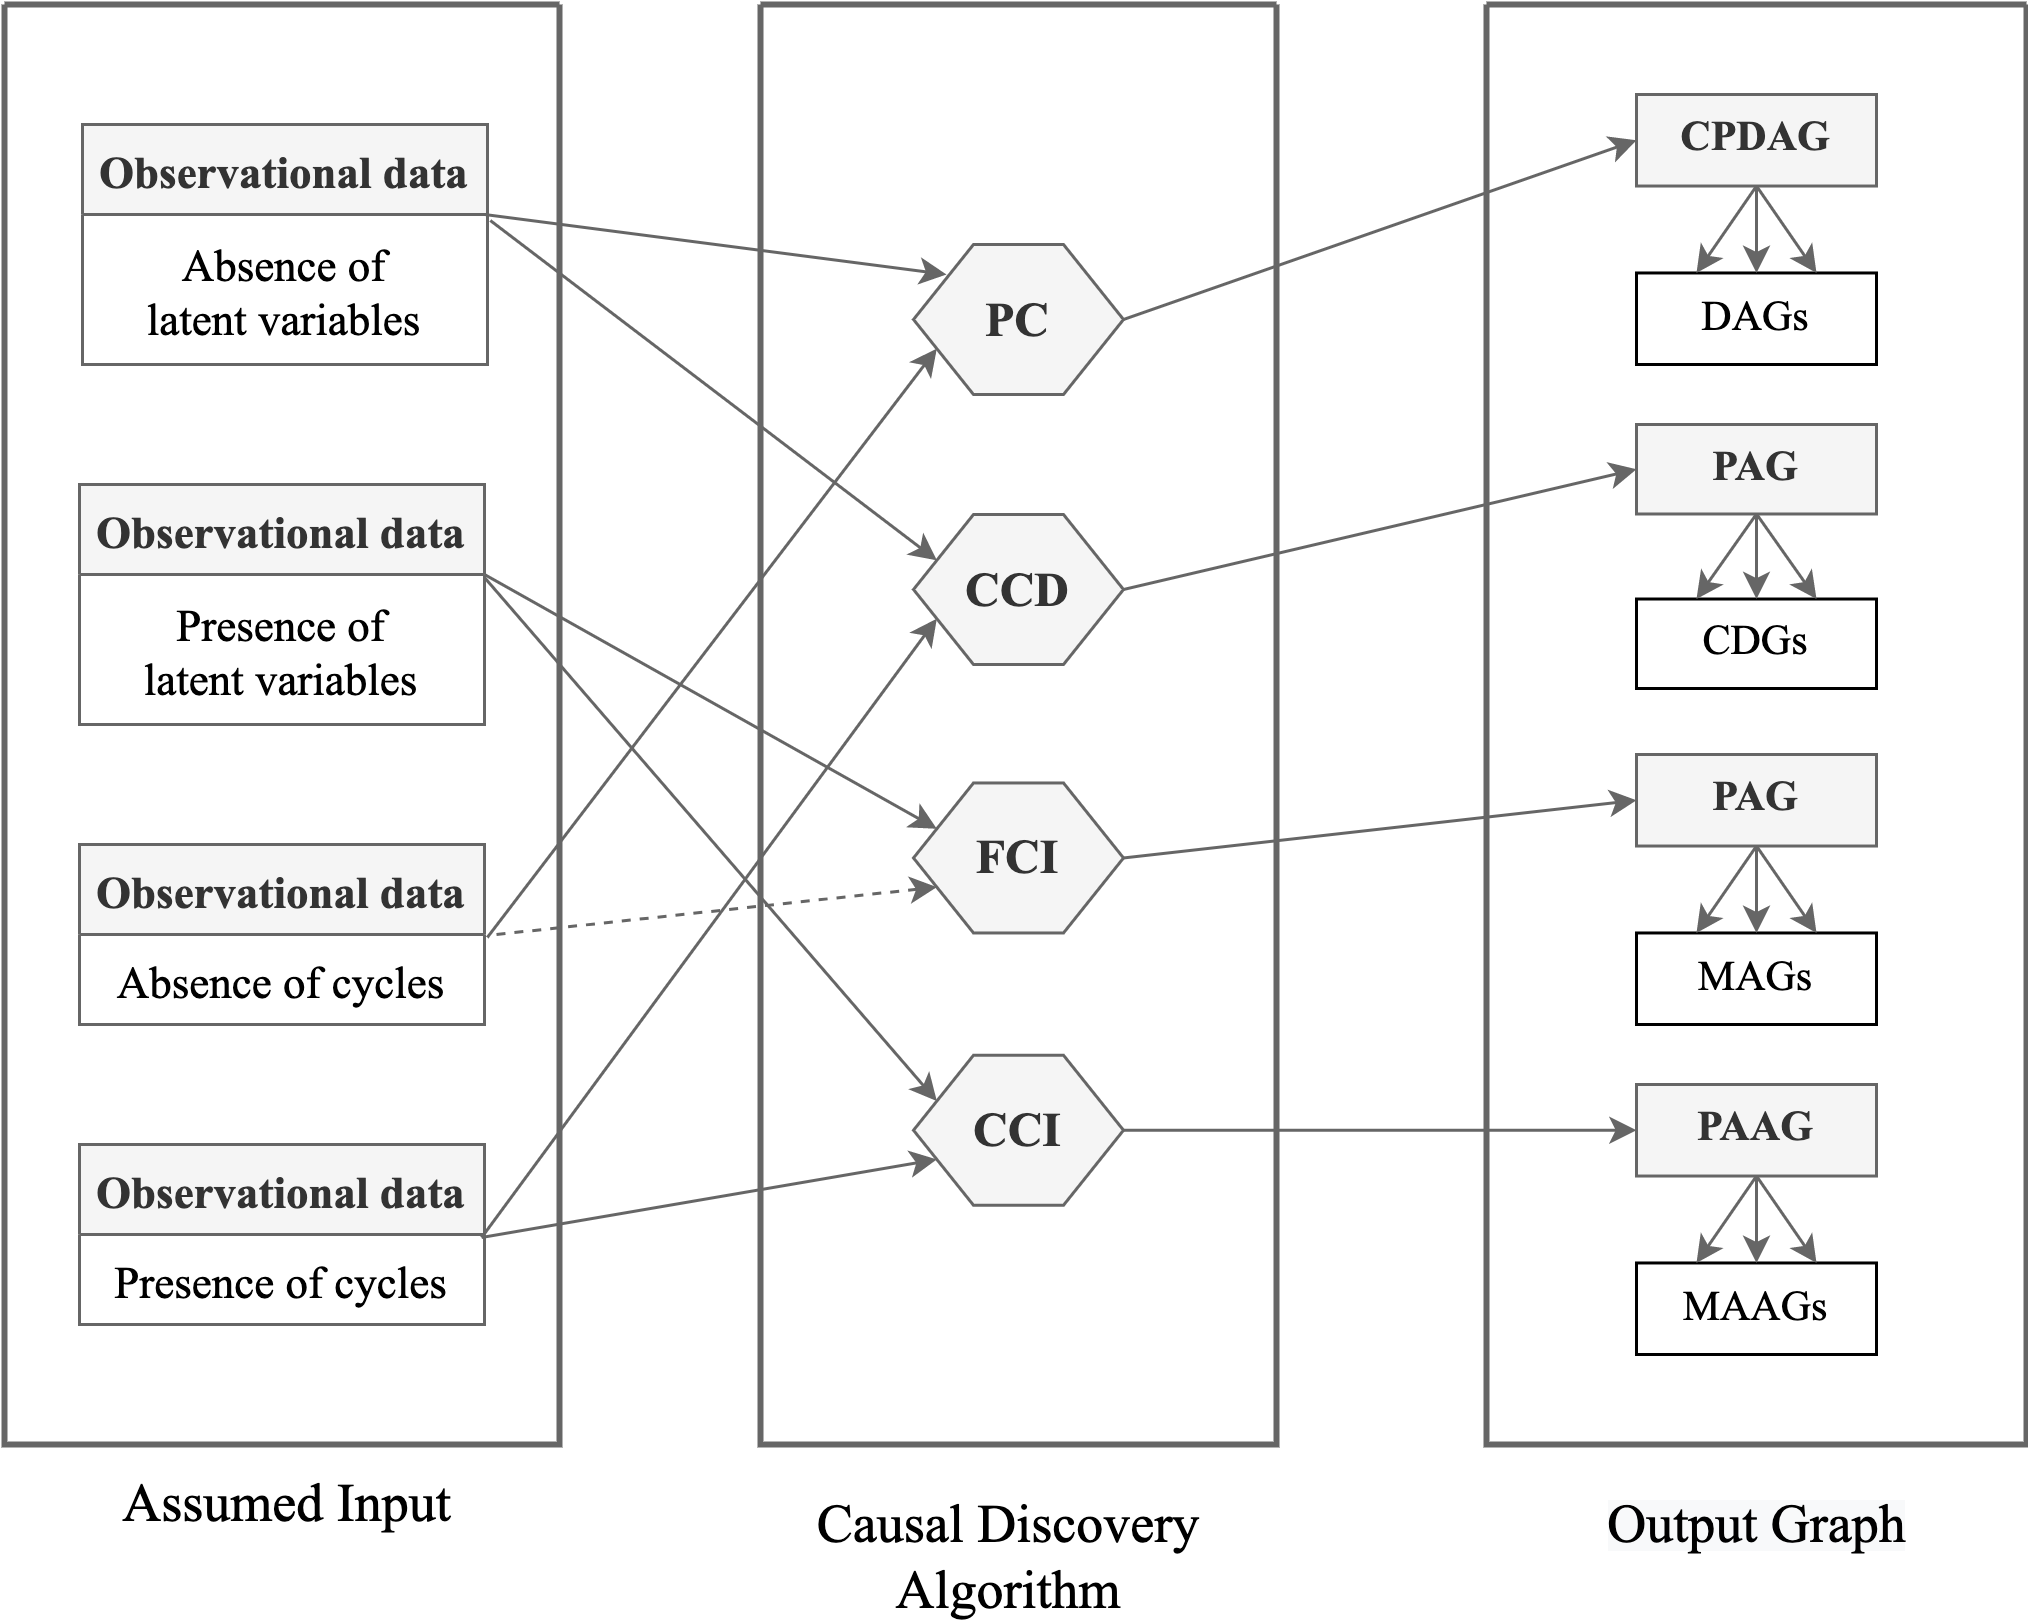
\includegraphics[width=.85\textwidth]{figures/landscape.png}
%         % \vspace{2mm}
%         % \caption*{\textit{Note.} Given the statistical independencies, CCD construct a partial ancestral graph (PAG), which represents features common to all directed cyclic graphs in the Markov equivalence class.}
%     \label{fig:5}
% \end{figure}

% restore original geometry
\clearpage
\restoregeometry

\pagebreak
\newgeometry{left=2.88cm,right=2.88cm,top=2.4cm,bottom=3cm}

\subsection{Simulation}

To evaluate the performance of the considered algorithms, we conduct a simulation study. In this section, we discuss the simulation design, data generating process, and evaluation metrics in detail.
% In addition, we will briefly introduce the empirical data on which we test the algorithms.


\subsubsection{Simulation Design}
We test each algorithm under different conditions by varying the number of variables (rows of \figref{6}) and the number of edges -- the density (columns of \figref{6}). We also evaluate the effect of an unobserved confounder by adding a latent variable ($L_1$ in \figref{6}). Lastly, we vary the sample size across the range we often encounter in psychological research; $n \in \{150, 500, 1000\}$ for every simulated cyclic model \citep{constantin2022}. Thus, it leads to a $2 \times 2 \times 2 \times 3$ design; number of variables $\times$ density $\times$ latent confounder (presence/absence) $\times$ sample size.

\vspace{2mm}

\begin{figure}[H]
    \centering
        \caption{Simulation settings.}
        \vspace{1mm}
        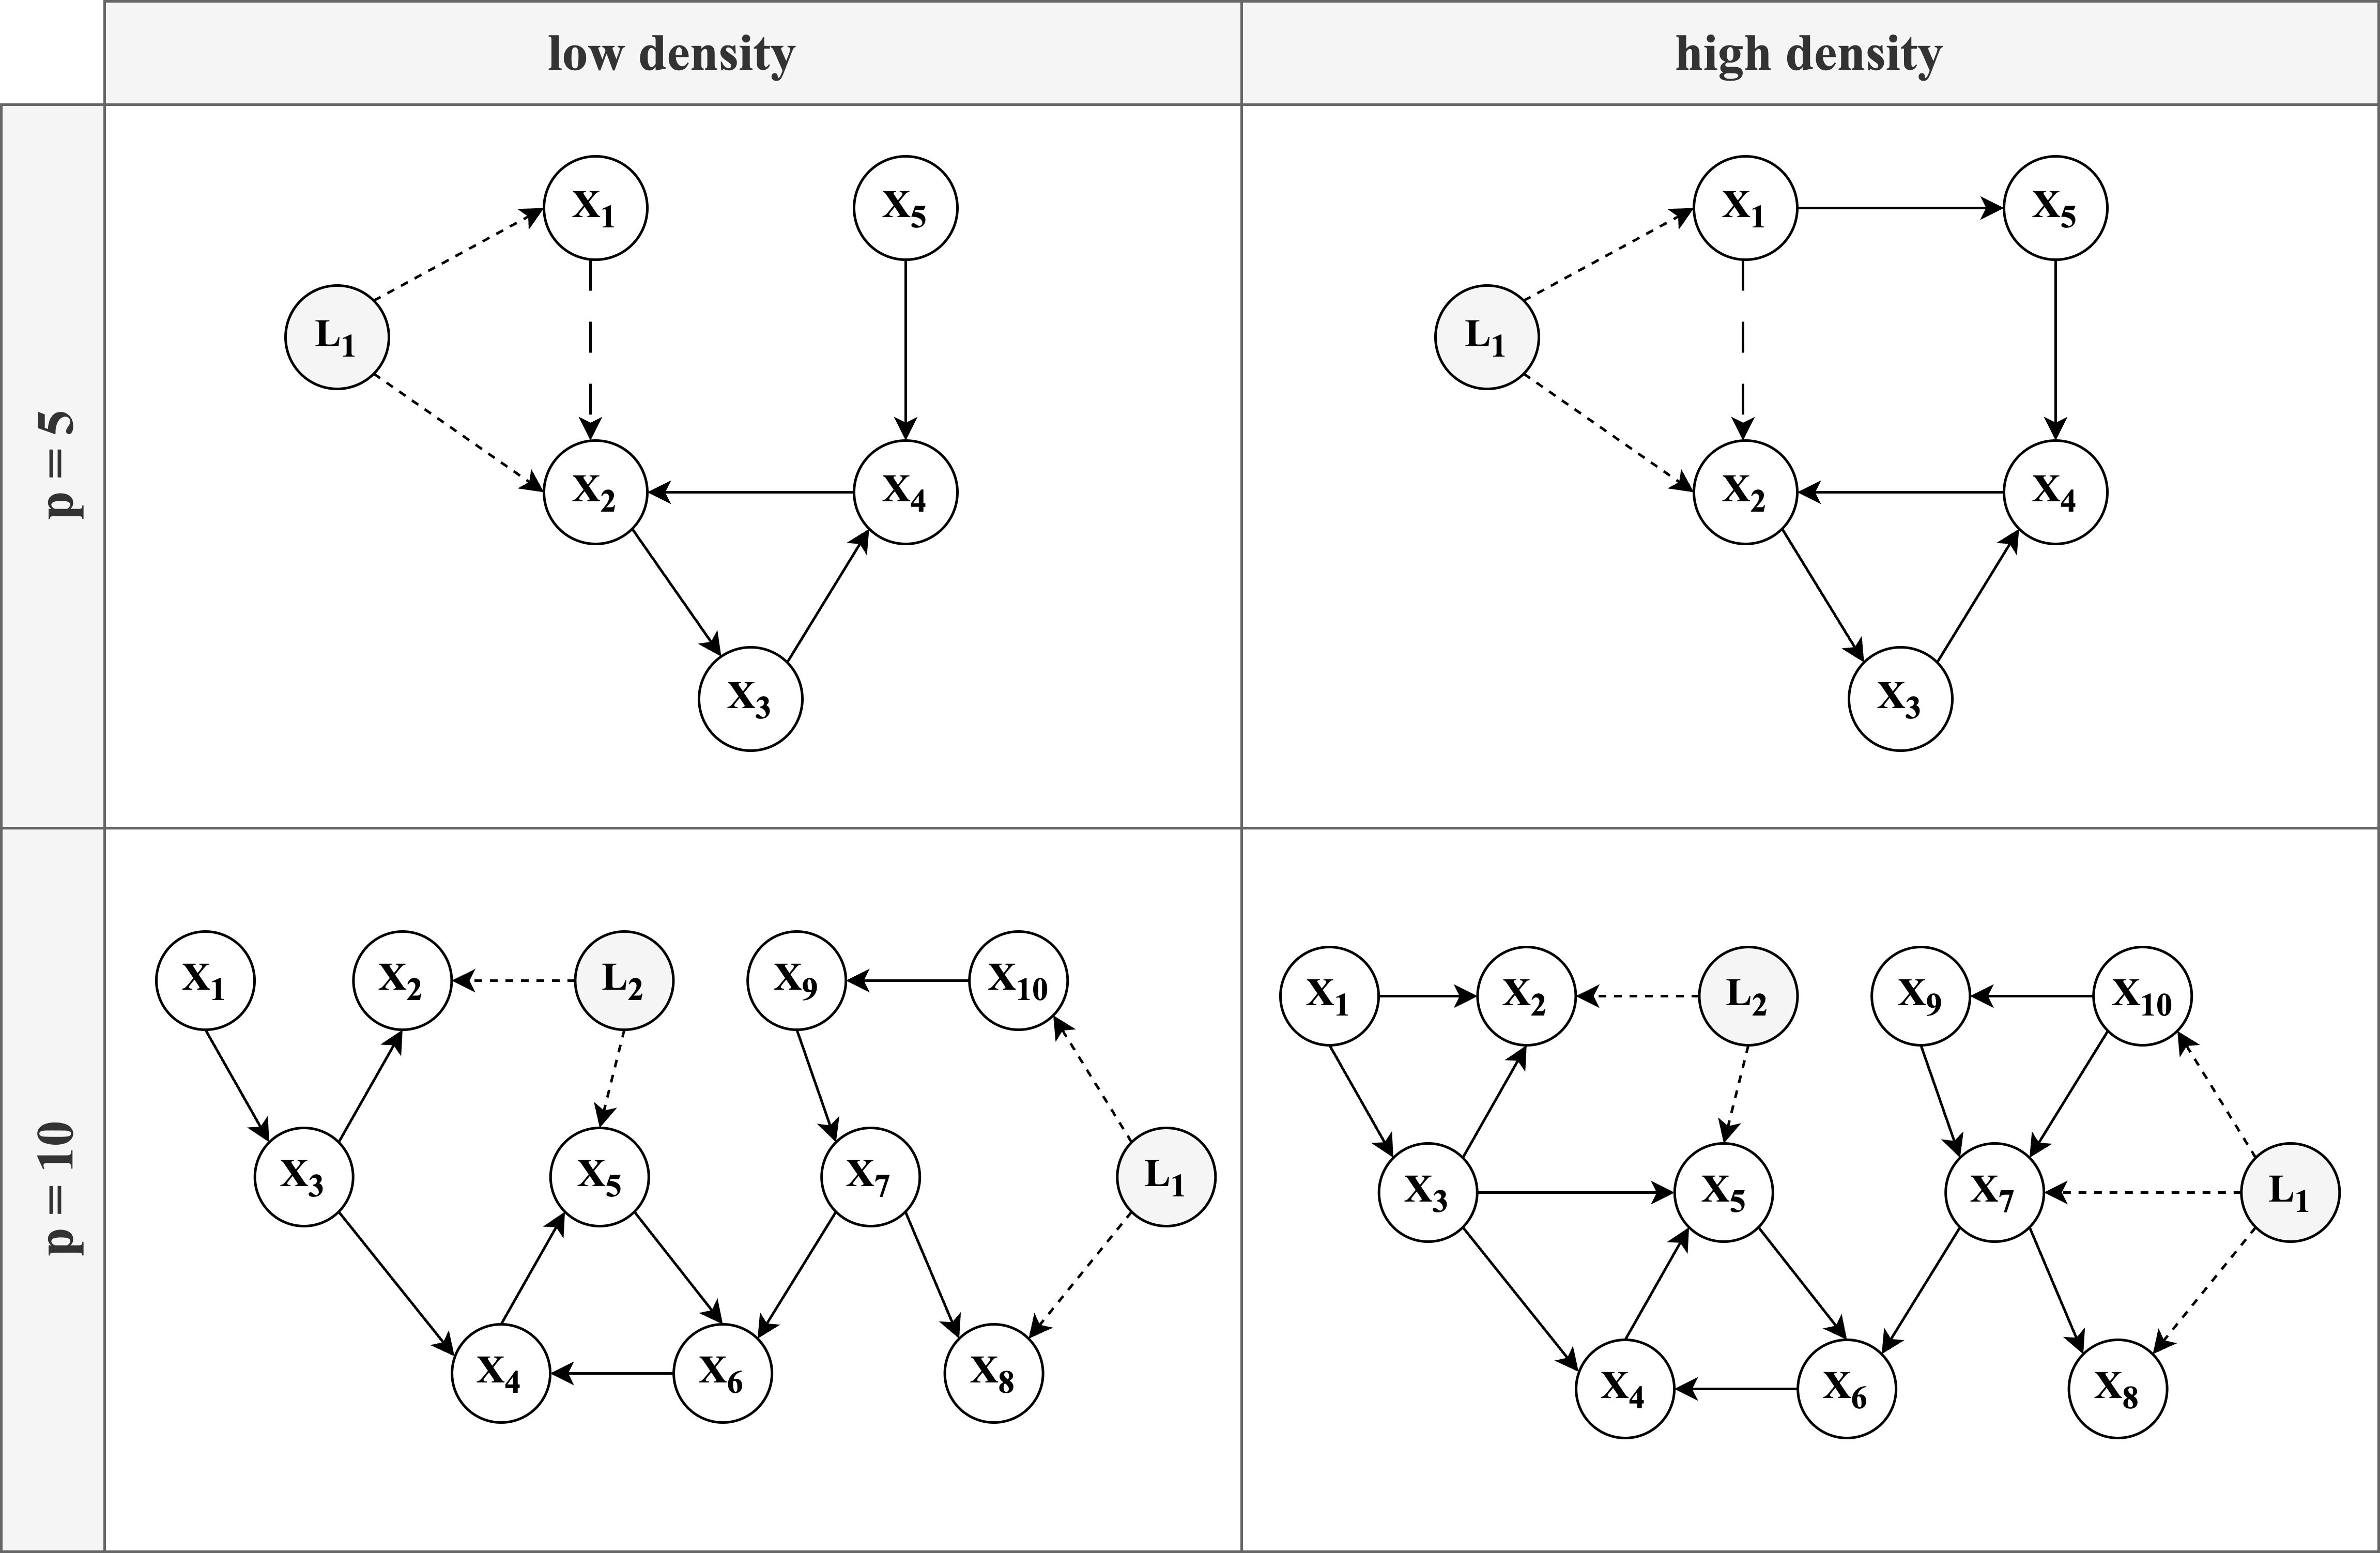
\includegraphics[width=1\textwidth]{figures/simsetting3.png}
        \vspace*{-4mm}
        \caption*{\small{\textit{Note.} We vary the number of variables: $p \in \{5, 10\}$, the density: high / low, the influence of a latent confounder ($L_1$): absence / presence, and the sample size: $n \in \{150, 500, 1000\}$, which results in a $2 \times 2 \times 2 \times 3$ simulation design.}}
    \label{fig:6}
\end{figure}

\vspace{-1cm}
% \newgeometry{left=2.88cm,right=2.88cm,top=2.8cm,bottom=2.8cm}
\subsubsection{Data Generation}
As illustrated above, we simulate data from different cyclic models, all of which are characterized by \textit{linear} relations and \textit{independent Gaussian} error terms. These types of models are often used in psychological research, and for such cyclic models, the global Markov property -- the necessary condition for constraint-based causal discovery -- also holds , as shown in section \ref{acyclicvscyclic}.

% Not only that they are commonly assumed in psychological research, but also under these assumptions, the requirement for using causal discovery methods -- global Markov property -- holds, as shown in section \ref{acyclicvscyclic}. 

To generate data, we first define a coefficient matrix $\mathbf{B}$ and sample the error terms ($\varepsilon$) from independent Gaussian distributions. After drawing the values of $\varepsilon$, we generate observations of $\mathbf{X}$ by solving the following equation: 
$\mathbf{X} = (\mathbf{I} - \mathbf{B})^{-1}\boldsymbol{\varepsilon},$
where $\mathbf{I}$ denotes the identity matrix. Note that this data generation scheme is possible provided that $(\mathbf{I} - \mathbf{B})$ is invertible, which is the case when the eigenvalues of $\mathbf{B}$ are smaller than one, $|\,\lambda\,| < 1$ \citep{eberhardt2010}. While this is guaranteed if $\mathbf{B}$ defines an acyclic model, for cyclic models, this does not always hold. Therefore, we check if this condition is satisfied for every cyclic model when specifying $\mathbf{B}$ matrix.
% and therefore requires careful specification of $\mathbf{B}$ matrices. 

% Note that the equations may not have unique solutions for some of the cyclic causal models. The necessary condition to have a unique solution is that $(\mathbf{I} - \mathbf{B})$ is invertible. In cyclic models, this condition is only satisfied when the absolute values of eigenvalues of $\mathbf{B}$ are smaller than one, $|\lambda| < 1$ \citep{eberhardt2010}. Hence, we ensure that the specified $\mathbf{B}$ matrix satisfies the aforementioned condition.

\subsubsection{Evaluation Metrics}
We assess the performance of each algorithm using both \textit{local} and \textit{global} evaluation metrics; at a local level, we look at the individual edge-endpoints and at a global level, we look at the graph structure as a whole. As the local metrics, we utilize \textit{precision}, \textit{recall}, and \textit{uncertainty rate}. 
\begin{align*}
Precision &= \frac{\text{True Positive}}{\text{True Positive } + \text{ False Positive}} \vspace{1mm} \\[1.1ex]
Recall &= \frac{\text{True Positive}}{\text{True Positive } + \text{ False Negative}} \\[1.1ex]
Uncertainty\, rate &= \frac{\text{Number of circle endpoints } (\circ)}{\text{Total number of edge-endpoints}}
\end{align*}

\noindent Precision reflects the prediction accuracy (i.e., out of all predicted cases, how many are correct), and recall reflects the retrieval rate (i.e., out of all true cases, how many are retrieved). There are in total four possibilities for each edge-endpoint in a resulting graph: no edge-endpoint (null), arrow head ($>$), arrow tail ($-$), and circle ($\circ$). Given that circle endpoints imply an algorithm is unsure of the direction of causal relations, the uncertainty rate is defined as a proportion of the circle endpoints occurred in an output.
For the other endpoints, we calculate the precision and recall. For example, for the arrow head, they are computed as: $precision =  \frac{a}{a + d + g}$ and $recall = \frac{a}{a + b + c}$ (see \autoref{tab:2}).

\vspace{1.5mm}
\begin{table}[H]
\begin{center}
\caption{Confusion matrix for the three types of edge-endpoints.}
\label{tab:2}
\begin{tabular}{@{}cc|ccc@{}}
\multicolumn{1}{c}{} &\multicolumn{1}{c}{} &\multicolumn{3}{c}{\textbf{Estimated endpoint}}\vspace{1mm} \\ 
\multicolumn{1}{c}{} & 
\multicolumn{1}{c|}{} & 
\multicolumn{1}{c}{Arrow head ($>$)} & 
\multicolumn{1}{c}{Arrow tail ($-$)} &
\multicolumn{1}{c}{\hspace*{4mm} Null \hspace*{4mm}} \\ 
\cline{2-5}
\multirow[c]{2}{*}{\rotatebox[origin=tr]{90}{\textbf{True endpoint}}}
& Arrow head ($>$)  & \textit{a} &  \textit{b} & \textit{c}   \\[1.5ex]
& Arrow tail ($-$)  & \textit{d}   & \textit{e} & \textit{f} \\[1.5ex]
& Null  & \textit{g} & \textit{h} & \textit{i} \\[1.5ex]
\end{tabular}
\end{center}
\smallskip
\small\textit{Note}. The true endpoints are presented in rows, and the estimated endpoints are presented in columns. There are in total four possible edge-endpoints that can occur in an output: arrow head, arrow tail, null (no endpoint), and circle. The circle endpoints ($\circ$), however, are not counted toward the calculation of \textit{precision} and \textit{recall} but are used for calculating the \textit{uncertainty rate}.

\end{table}

\clearpage
\restoregeometry


% \vspace{2mm}
As the global metric, we use \textit{structural Hamming distance} (SHD) \citep{de2009comparison}. SHD quantifies the level of differences between two graphs by counting the number of edge insertions, deletions, and direction changes required to move from one graph (estimated graph $\hat{\mathcal{G}}$) to the other (true graph $\mathcal{G}$). It can be formulated as:
$\textit{SHD} = A + D + C,$
where $A$, $D$, and $C$ represent, respectively, the number of added edges, deleted edges, and direction changes. Thus, the smaller the SHD value is, the more similar $\hat{\mathcal{G}}$ is to $\mathcal{G}$, indicating that an algorithm recovers the true graph well.



% also pcalg has a function for computing SHD. 



% possible stuff to omit in the report:
% - compared to oracel graph, maybe we can add it to the final report?
% - testing on empirical data.. --> to the final report?





\clearpage
\bibliography{references} 
\nocite{*}




\pagebreak
\newgeometry{left=3.9cm,right=3.9cm,top=3cm,bottom=3cm}

\begin{appendices} 

\section{CCD Details}\label{algCCD}

%% CCD algorithm %%
\begin{algorithm} 
\caption{Cyclic Causal Discovery (CCD)}
 
 % input
 \hspace*{\algorithmicindent} \textbf{Input:} A conditional independent oracle for a distribution $\mathcal{P}$, satisfying global directed Markov property and faithfulness conditions with respect to a directed graph $\mathcal{G}$ with vertex set $\mathcal{V}$. 

 % output
 \hspace*{\algorithmicindent} \textbf{Output:} A PAG $\Psi$ for the Markov equivalence class $\text{Equiv}(\mathcal{G})$.
 
\begin{algorithmic}[1]
% step 1
\State \textit{\textbf{Step 1.}}\label{ccdstep1} Form a complete graph ($\Psi$) with the edge $\multimapboth$ between every pair of vertices in $\mathcal{V}$.
    \State $n = 0$
    \Repeat
        \Repeat
            \State \multiline{Select an ordered pair of variables $X$ and $Y$ that are adjacent in $\Psi$ such that the number of vertices in $\mathbf{Adjacent}(\Psi ,X)\backslash\{Y\} \ge n$, and select a subset $\mathcal{S}$ of $\mathbf{Adjacent}(\Psi ,X) \backslash \{Y\}$ with $n$ vertices. \\
            If $X \indep Y \mid \mathcal{S}$, then delete the edge $X \multimapboth Y$ and record $\mathcal{S}$ in $\mathbf{Sepset} \langle X,Y \rangle$ and $\mathbf{Sepset}\langle X,Y \rangle$.}
            \vspace{.1mm}
        \Until{ \multiline{all pairs of adjacent variables $X$ and $Y$ such that  the number of vertices in $\mathbf{Adjacent}(\Psi ,X)\backslash\{Y\} \ge n$ and all sets $\mathcal{S}$ such that the number of vertices in $\mathcal{S} = n$ have been tested.\\
        $n = n + 1;$}}
        \vspace{.1mm}
    \Until{ for all ordered pairs of adjacent vertices $X$ and $Y$, $\mathbf{Adjacent}(\Psi ,X)\backslash\{Y\} < n$}.

% step 2
\State \textit{\textbf{Step 2.}} \label{ccdstep2} For each triple of vertices $A, B, C$ such that each of the pair of $A, B$ and the pair $B, C$ are adjacent in $\Psi$ but the pair $A, C$ are not adjacent in $\Psi$, then:
    \State (i) orient $A *-*B*-*C$ as $A \rightarrow B \leftarrow C$ \textit{iff} $B \notin \mathbf{Sepset}\langle A, B \rangle$.
    \State (ii) orient $A *-*B*-*C$ as $A *-* \underline{B}*-*C$ \textit{iff} $B \in \mathbf{Sepset}\langle A, B \rangle$.

% step 3
\State \textit{\textbf{Step 3.}} \label{ccdstep3} For each triple of vertices $A, X, Y$ in $\Psi$ such that (a) $A$ is not adjacent to $X$ or $Y$, (b) $X$ and $Y$ are adjacent, (c) $X \notin \mathbf{Sepset}\langle A, Y \rangle$ , then orient $X *-* Y$ as $X \leftarrow Y$ if $A \nindep X \mid \mathbf{Sepset}\langle A, Y \rangle$.

% step 4
\State \textit{\textbf{Step 4.}}  \label{ccdstep4} For each vertex $V$ in $\Psi$ form the following set: $X \in \mathbf{Local}(\Psi, V)$ or there is a vertex $Y$ such that $X \rightarrow Y \leftarrow V$ in $\Psi$.
\State $m = 0$
    \Repeat
        \Repeat 
            \State \multiline{Select an ordered triple $\langle A, B, C \rangle$ such that $A \rightarrow B \leftarrow C$, $A$ and $C$ are not adjacent, and $\mathbf{Local}(\Psi, A) \backslash \{B, C\}$ has $\ge m$ vertices.\\
            Select a set $T \subseteq \mathbf{Local}(\Psi, A) \backslash \{B, C\}$ with $m$ vertices. If $A \indep C \mid T \cup \{B\}$, then orient $A \rightarrow B \leftarrow C$ as $A \rightarrow \udensdot{B} \leftarrow C$ and record $T \cup \{B\}$ in $\mathbf{Supset} \langle A, B, V \rangle$.}
            \vspace{.1mm}

\algstore{myccd}
\end{algorithmic}
\end{algorithm}

\begin{algorithm}                     
\begin{algorithmic} [1]       % enter the algorithmic environment
\algrestore{myccd}
        \Until \multiline{for all triples such that $A \rightarrow B \leftarrow C$ (not $A \rightarrow \udensdot{B} \leftarrow C$), $A$ and $C$ are not adjacent, $\mathbf{Local}(\Psi, A) \backslash \{B\}$ has $\ge m$ vertices, every subset $T$ with $m$ vertices has been considered.}
        \vspace{.1mm}
        
        \State $m = m + 1;$
    \Until \multiline{all ordered triples $\langle A, B, C \rangle$ such that $A \rightarrow B \leftarrow C$, $A$ and $C$ are not adjacent, are such that $\mathbf{Local}(\Psi, A) \backslash \{B\}$ have $< m$ vertices.}
\vspace{.1mm}

% step 5
\State \textit{\textbf{Step 5.}} \label{ccdstep5} If there is a quadruple $A$, $B$, $C$, $D$ in $\Psi$ of distinct vertices such that:\\ 
(i) $A \rightarrow \udensdot{B} \leftarrow C$,\\
(ii) $A \rightarrow D \leftarrow C$ or $A \rightarrow \udensdot{D} \leftarrow C$,\\
(iii) $B$ and $D$ are adjacent,\\
then orient $B *-* D$ ad $B \rightarrow D$ in $\Psi$ if $D \notin \mathbf{Subset}\langle A, B, C \rangle$. Else orient $B *-* D$ as $B *- D$ in $\Psi$.

% step 6
\State \textit{\textbf{Step 6.}}  \label{ccdstep6} For each quadruple $A$, $B$, $C$, $D$ in $\Psi$ of distinct vertices such that:\\
    (i) $D$ is not adjacent to both $A$ and $C$,\\
    (ii) $A \rightarrow \udensdot{B} \leftarrow C$,\\
    if $A \nindep D \mid \mathbf{Supset} \langle A, B, C \rangle \cup \{D\}$,
    then orient $B *-* D$ as $B \rightarrow D$ in $\Psi$.
\end{algorithmic}
\end{algorithm}

\pagebreak
\vspace*{1mm}
\section{FCI Details}\label{algFCI}
%% FCI algorithm %%

\begin{algorithm} 
\caption{Fast Causal Inference (FCI)}
 % input
 \hspace*{\algorithmicindent} \textbf{Input:} A conditional independent oracle for a distribution $\mathcal{P}$, satisfying global directed Markov property and faithfulness conditions with respect to a directed graph $\mathcal{G}$ with vertex set $\mathcal{V}$.\\
 % output
 \hspace*{\algorithmicindent} \textbf{Output:} A PAG $\mathcal{\hat{G'}}$ for the Markov equivalence class of MAGs ($\text{Equiv}(\mathcal{G})$).


\begin{algorithmic}[1]
% step 1
\State \textit{\textbf{Step 1.}}\label{fcistep1} Form the complete undirected graph $Q$ on the vertex set $\mathcal{V}$.

    \State $n = 0$
    \Repeat
        \Repeat
            \State \multiline{Select an ordered pair of variables $X$ and $Y$ that are adjacent in $Q$ such that the number of vertices in $\mathbf{Adjacent}(Q ,X)\backslash\{Y\} \ge n$, and select a subset $\mathcal{S}$ of $\mathbf{Adjacent}(Q ,X) \backslash \{Y\}$ with $n$ vertices. \\
            If $X \indep Y \mid \mathcal{S}$, then delete the edge $X \multimapboth Y$ and record $\mathcal{S}$ in $\mathbf{Sepset} \langle X,Y \rangle$ and $\mathbf{Sepset}\langle X,Y \rangle$.}
            \vspace{.1mm}
        \Until{ \multiline{all pairs of adjacent variables $X$ and $Y$ such that  the number of vertices in $\mathbf{Adjacent}(Q ,X)\backslash\{Y\} \ge n$ and all sets $\mathcal{S}$ such that the number of vertices in $\mathcal{S} = n$ have been tested.\\
        $n = n + 1;$}}
        \vspace{.1mm}
    \Until{ for all ordered pairs of adjacent vertices $X$ and $Y$, $\mathbf{Adjacent}(Q ,X)\backslash\{Y\} < n$}.

\algstore{myfci}
\end{algorithmic}
\end{algorithm}


\begin{algorithm}                     
\begin{algorithmic}[1]     
\algrestore{myfci}

% step 2
\State \textit{\textbf{Step 2.}} \label{fcistep2} Let $Q'$ be the undirected graph resulting from step 1. For each triplet $\langle A, B, C \rangle$ such that each of the pair of $A, B$ and the pair $B, C$ are adjacent in $Q'$ but the pair $A, C$ are not adjacent in $Q'$, then:
    \State (i) orient $A *-*B*-*C$ as $A \rightarrow B \leftarrow C$ \textit{iff} $B \notin \mathbf{Sepset}\langle A, B \rangle$.
    \State (ii) orient $A *-*B*-*C$ as $A *-* \underline{B}*-*C$ \textit{iff} $B \in \mathbf{Sepset}\langle A, B \rangle$.
    
% step 3
\State \textit{\textbf{Step 3.}} \label{fcistep3} For each pair of variables $A$ and $B$ adjacent in $Q'$, if $A$ and $B$ are d-separated given any subset $S$ of $\textbf{Possible-d-sepset} \langle A, B \rangle) \backslash \{A, B\}$ or any subset $S$ of $\textbf{Possible-d-sepset} \langle B, A \rangle) \backslash \{A, B\}$ in $Q'$, then remove the edge between $A$ and $B$, and record $\mathcal{S}$ in $\mathbf{Sepset} \langle A, B \rangle$ and $\mathbf{Sepset}\langle B, A \rangle$.

% step 4
\State \textit{\textbf{Step 4.}}  \label{fcistep4} Reorient an edge between any pair of variables $X$ and $Y$ ($X \multimapboth Y$) following the orientation rules below. 
\Repeat
        \If{there is a directed path from $A$ to $B$, and an edge $A * - * B$} 
            \State orient $A * - * B$ as $A * \rightarrow B$,
        
        \ElsIf{$B$ is a collider along $\langle A, B, C \rangle$, $B$ is adjacent to $D$, and $D \in \mathbf{Sepset}\langle A, C \rangle$} 
            \State orient $B*-*D$ as $B \leftarrow * D$,
        
        \ElsIf{$U$ is a definite discriminating path between $A$ an d $B$ for $M$ in the path $\prod$, and $P$ and $R$ are adjacent to $M$ on $U$, and $P - M - R$ is a triangle} 
                \If{$M \in \mathbf{Sepset}\langle A, B \rangle$} {$M$ is marked as non-collider on subpath $P *-* \underline{M} *-* R$}
                \Else { $P*-*M*-*R$ is oriented as $P* \rightarrow M \leftarrow * R$.}
                \EndIf
        
        \ElsIf{$P *\rightarrow \underline{M} *-* R$} 
            \State orient as $P * \rightarrow M \rightarrow R$.
    \EndIf
\Until{no more edges can be oriented.}

\end{algorithmic}
\end{algorithm}


%% orientation rule from Zhang 2008 %%
% The orientation rules are as follows: (ref. Zhang 2008)

% \begin{enumerate}[nolistsep, label=(\roman*)] 

%     \item If $A *\rightarrow B \multimapinv * C$ and $A$ and $C$ are not adjacent, then orient the triplet as $A *\rightarrow B \rightarrow C$.

%     \item If $A \rightarrow B *\rightarrow C$ or $A *\rightarrow B \rightarrow C$ and $A * \multimap C$, then orient $A *\multimap C$ as $A *\rightarrow C$.

%     \item If $A *\rightarrow B \leftarrow* C$ and $A *\multimap D \multimapinv *C$, and $A$ and $D$ are not adjacent while $D * \multimap B$, then orient $D *\multimap B$ as $D *\rightarrow B$.

%     \item If $u = \langle D,...,A,B,C \rangle$ is a discriminating path between D and C with respect to B, and $B \multimapinv* C$; then if $B \in \mathbf{Sepset} \langle D, C \rangle$, orient $B \multimapinv C$ as $B \rightarrow* C$; otherwise orient the triplet $\langle A, B, C \rangle$ as $A \leftrightarrow B \leftrightarrow C$.
% \end{enumerate}


\pagebreak
\section{CCI Details}\label{algCCI}

%% CCI algorithm %%

\begin{algorithm} 
\caption{Cyclic Causal Inference (CCI)}
 % input
 \hspace*{\algorithmicindent} \textbf{Input:} A conditional independent oracle for a distribution $\mathcal{P}$, satisfying global directed Markov property and faithfulness conditions w.r.t. a directed graph $\mathcal{G}$ with vertex set $\mathcal{V}$. ($\mathcal{V} = \mathbf{O} \cup \mathbf{L} \cup \mathbf{S}$), where $\mathbf{O}$, $\mathbf{L}$, and $\mathbf{S}$ refer to the sets of observable, latent, and selection variables, respectively.\\
 % output
 \hspace*{\algorithmicindent} \textbf{Output:} A PAAG ($\mathcal{\hat{G'}}$) for the Markov equivalence class of MAAGs ($\text{Equiv}(\mathcal{G})$).


\begin{algorithmic}[1]
% step 1
\State \textit{\textbf{Step 1.}}\label{ccistep1} Run FCI's skeleton discovery procedure.

% step 2
\State \textit{\textbf{Step 2.}} \label{ccistep2} Run FCI's collider structure (v-structure) orientation procedure.

% step 3
\State \textit{\textbf{Step 3.}} \label{ccistep3} For any triplet $\langle O_i, O_k, O_j \rangle$, such that we have $O_k \multimapinv* O_i$, if $O_i \indep_\mathcal{G} O_j \mid \mathbf{Sepset} \langle O_i, O_j \rangle \cup \mathbf{S}, \text{where } \mathbf{Sepset} \langle O_i, O_j \rangle$ is a separating set discovered in step 1, $O_k \notin \mathbf{Sepset} \langle O_i, O_j \rangle$, $O_i \nindep_\mathcal{G} O_k \mid \mathbf{Sepset} \langle O_i, O_j \rangle \cup \mathbf{S}$ and $O_j \nindep_\mathcal{G} O_k \mid \mathbf{Sepset} \langle O_i, O_j \rangle \cup \mathbf{S}$, then orient $O_k \multimapinv* O_i$ as $O_k \leftarrow* O_i$.

% step 4
\State \textit{\textbf{Step 4.}}  \label{ccistep4} Find additional non-minimal d-separating sets.

\State $m = 0$
    \Repeat
        \Repeat
            \State \multiline{Select an ordered triplet $\langle O_i, O_j, O_k \rangle$ with the collider structure $O_i *\rightarrow O_j \leftarrow* O_k$ such that $|\textbf{PD-Sep}(O_i)| \ge m$}
            \vspace{.1mm}
            \Repeat
            \State \multiline{Select a subset\\
            $\mathbf{W} \subseteq \textbf{PD-Sep}(O_i) \backslash \{\mathbf{Sepset} \langle O_i, O_k \rangle \cup \{O_j, O_k \} \}$ with $m$ vertices \\
            $\mathbf{T} = \mathbf{W} \cup \mathbf{Sepset} \langle O_i, O_k \rangle \cup O_j$\\
            if $O_i$ and $O_k$ are d-separated given $\mathbf{T} \cup \mathbf{S}$, then record the set $\mathbf{T}$ in $\mathbf{Supset} \langle O_i, O_j, O_k \rangle$
            }
            \vspace{.1mm}

        \Until {\multiline{all subsets\\
        $\mathbf{W} \subseteq \textbf{PD-Sep}(O_i) \backslash \{\mathbf{Sepset} \langle O_i, O_k \rangle \cup \{O_j, O_k \} \}$ have been considered or a d-separating set of $O_i$ and $O_k$ has been recorded in $\mathbf{Supset} \langle O_i, O_j, O_k \rangle$;}}
        \vspace{.1mm}
        
    \Until{ \multiline{all triplets $\langle O_i, O_j, O_k \rangle$ with the collider structure $O_i *\rightarrow O_j \leftarrow* O_k$ and $|\textbf{PD-Sep}(O_i)| \ge m$ have been selected;}}
    \vspace{.1mm}

\Until{ \multiline{all ordered triplets $\langle O_i, O_j, O_k \rangle$ with the collider structure $O_i *\rightarrow O_j \leftarrow* O_k$ have $|\textbf{PD-Sep}(O_i)| < m$;}}
\vspace{.1mm}

% step 5
\State \textit{\textbf{Step 5.}} \label{ccistep5} Find all quadruples of vertices $ \langle O_i, O_j, O_k, O_l \rangle$ such that $O_i$ and $O_k $ are non-adjacent, $O_i *\rightarrow O_l \leftarrow* O_k$, and $O_i \indep_\mathcal{G} O_k \mid \mathbf{W} \cup \mathbf{S}$ with $O_j \in \mathbf{W}$ and $\mathbf{W} \subseteq \mathbf{O} \backslash \{O_i, O_k \}$. If $O_l \notin \mathbf{W} = \mathbf{Sepset} \langle O_i, O_k \rangle$ as discovered in step 2, then orient $O_j * \multimap O_l$ as $O_j *\rightarrow O_l$. If we also have $O_i *\rightarrow O_j \leftarrow* O_k$ and $O_l \in \mathbf{W} = \mathbf{Supset} \langle O_i, O_j, O_k \rangle$ as discovered in step 4, then orient $O_j * \multimap O_l$ as $O_j *- O_l$.

\algstore{mycci}
\end{algorithmic}
\end{algorithm}


\begin{algorithm}                     
\begin{algorithmic}[1]     
\algrestore{mycci}

% step 6
\State \textit{\textbf{Step 6.}}  \label{ccistep6} For any two vertices $O_i$ and $O_k$, if we have $O_i \indep_\mathcal{G} O_k \mid \mathbf{W} \cup \mathbf{S}$ for some $\mathbf{W} \subseteq \mathbf{O} \backslash \{ O_i, O_k \}$ discovered in step 1 or step 4 with $O_j \in \mathbf{W}$ but we have $O_i \nindep_\mathcal{G} O_k \mid O_l \cup \mathbf{W} \cup \mathbf{S}$, then orient $O_l \multimapinv* O_j$ as $O_l \leftarrow * O_j$.

% step 7
\State \textit{\textbf{Step 7.}}  \label{ccistep7} Execute orientation rules until no more endpoints can be oriented. The orientation rules are as follows:
\begin{enumerate}[nolistsep, label=(\roman*)] 
    \item If we have $O_i * \rightarrow O_j \multimapinv * O_k$ with $O_i$ and $O_k$ non-adjacent, then orient $O_j \multimapinv * O_k$ as $O_j - * O_k$. Furthermore, if $O_i *\rightarrow O_j$ is not potentially 2-triangulated w.r.t. $O_k$, then orient $O_j \multimap O_k$ as $O_j \rightarrow O_k$.

    \item If we have $O_i -* O_j \multimapinv* O_k$ with $O_i$ and $O_k$ non-adjacent, and $O_j \multimapinv O_k$ is not potentially 2-triangulated w.r.t. $O_i$, then orient $O_j \multimapinv* O_k$ as $O_j -* O_k$.

    \item Suppose we have $O_i * \rightarrow O_j - O_k$ with $O_i$ and $O_k$ non-adjacent, and $O_i * \rightarrow O_j$ is potentially 2-triangulated w.r.t. $O_k$. If $O_i * \rightarrow O_j$ can be potentially 2-triangulated w.r.t. $O_k$ using only one vertex $O_l$ in the triangle involve $\{O_i, O_j, O_l \}$, then orient $O_i * \multimap O_l$ as $O_i * \rightarrow O_l$, $O_j \multimapinv * O_l$ as $O_j * \rightarrow O_l$ and/or $O_j * \multimapinv O_l$ as $O_j *- O_l$. Next, if there exists only one potentially undirected path $\prod_{O_l, O_k}$ between $O_l$ and $O_k$, then substitute all circle endpoints on $\prod_{O_l, O_k}$ with tail endpoints ($-$).

    \item If $O_i * \rightarrow O_j -* O_k$, there exists a path $\prod = \langle O_k, ..., O_i \rangle$ with at least $n \ge 3$ vertices such that we have $O_h -* O_{h+1}$ for all $ 1 \le i \le n -1$, and we have $O_1 \multimapinv * O_n$, then orient $O_1 \multimapinv * O_n$ as $O_1 - * O_n$.

    \item If we have the sequence of vertices $\langle O_1, ..., O_n \rangle$ such that $O_i -* O_{i+1}$ with $1 \le i \le n-1$, and we have $O_1 \multimapinv* O_n$, then orient $O_1 \multimapinv * O_n$ as $O_1 -* O_n$.

    \item If we have $O_k * \multimap O_i$, there exists a non-potentially 2-triangulated path $\prod = \langle O_i, O_j, O_l, ..., O_k \rangle$ such that $O_k * \multimap O_i$ is not potentially 2-triangulated w.r.t. $O_j$, and $O_j *-* O_i *-* O_k$ is an unshielded non-v-structure, then orient $O_k * \multimap O_i$ as $O_k *- O_i$.

    \item Suppose we have $O_i \multimapinv O_k, O_i -* O_k *- O_l$, a non-potentially 2-triangulated path $\prod_1$ from $O_i$ to $O_j$, and a non-potentially 2-triangulated path $\prod_2$ from $O_i$ to $O_l$. Let $O_m$ be a vertex adjacent to $O_i$ on $\prod_1$, and let $O_n$ be the vertex adjacent to $O_i$ on $\prod_2$. If further $O_m *-* O_i *-* O_n$ is an unshielded non-v-structure and $O_i \multimapinv * O_k$ is not potentially 2-triangulated w.r.t. both $O_n$ and $O_m$, then orient $O_i \multimapinv * O_k$ as $O_i -* O_k$.

    
\end{enumerate}


\end{algorithmic}
\end{algorithm}

\end{appendices}

\end{document}
 